
\documentclass[18pt, oneside]{book}

\usepackage[margin=1in]{geometry}
\usepackage{graphicx} % Required to insert images
\usepackage{placeins} %Required for floating help
\usepackage{hyperref}
\usepackage{amsmath}
\usepackage{amssymb}
\usepackage[toc,page]{appendix}
\usepackage{subfigure}
\usepackage{verbatim}
\usepackage{multirow}
\usepackage{adjustbox}
\setlength{\parindent}{0in}
\usepackage{multirow}
\usepackage{units}
\usepackage{soul}
\usepackage{fontspec}
\usepackage{cancel}
%\usepackage{times}
\fontseries{m}
\fontshape{it}
\fontsize{15}{18}


\newcommand{\mystar}{{\fontfamily{lmr}\selectfont$\star$}}

\bibliographystyle{plain}
\begin{document}

\begin{center}

\vspace*{3cm}
\Huge\bf The Campbell-Goldmann Collection \\
\vspace*{1cm}
\huge \bf The Gloop Edition


\par\noindent \vspace*{2cm}


\Large\bf Ute Goldmann  \\
Katriona Goldmann \\
Paul Campbell \\
Nicola Goldmann \\
\vspace*{0.5cm}   \today                               
\end{center}
\vspace*{5mm}
\thispagestyle{empty}



\tableofcontents

\part{Dips, Sauces and Accompaniments}
\setcounter{chapter}{1}

\section{Avocado Salsa}
\textbf{Ingredients} \\
1 ripe avocado \\
1 red chili, de-seeded and finely chopped \\
1 teaspoon chopped fresh corriander \\
1 teaspoon finely chopped ginger \\
2 tomatoes concasse \\
1 tablespoon thai fish sauce \\
Pinch of salt \\
zest and juice of half a lime \\

Half the avocado and remove the stone. Half again and remove skin. Chop into chunks. Place in a mixing bowl and add the rest if the ingredients.  Mix well and leave at room temperature for 30 mins for flavours to develop. 

\section{Chocolate Sauce}
\bf{Ingredients} \normalfont \\
55g butter \\
115g caster sugar \\ 
175ml water \\
175g good quality plain chocolate \\
1 tsp vanilla extract \\ 

Place all the ingredients in a small pan and gently heat stirring until melted. 

\section{Dad's Roasted Potatoes}
\bf{Ingredients} \normalfont \\
New potatoes \\
krauter saltz \\
princh of salt \\
dash of olive oil \\

Preheat the oven to 220$^\circ$. Par boil the potatoes for around 4 minutes. Add a covering of oil to a roasting tray and coat the potatoes with it. Add rosmary (krauter) salt and pepper. Place in the oven for \textit{at least} 40 minutes. 

\section{Guacamole}
\label{guacamole}
\subsection*{Rosi's Version}

\bf{Ingredients} \normalfont \\
1-2 ripe Avocadoes (firm to touch. Not squeedgy or hard) \\
Salt, Pepper \\
1 clove garlic \\
5 cherry tomatoes, quartered \\
Lemon Juice \\

Half the Avocado, ease out the stone then scoop the flesh out with a Tablespoon. Be thorough as the flesh just under the skin gives the lovely green colour. \\

Sqidge the flesh  (of the avocado not your cooking pal) into a bowl, add everything else adjust the seasoning and enjoy.

\subsection*{Ute's Version}

\bf{Ingredients} \normalfont \\
1-2 ripe Avocadoes (firm to touch. Not squeedgy or hard) \\
Salt, Pepper \\
1 pot of Cr\`{e}me Fraiche (diet if you must) \\
Sherry vinegar to taste \\
Dash of tabasco \\




\section{Roasted Sweet Potato Wedges}
\bf{Ingredients} \normalfont \\
Sweet potatoes \\
cumin \\
princh of salt \\
dash of olive oil \\
optional: flavoured mayonnaise \\

Cut the sweet potatoes into wedges, then toss in some olive oil, cumin and salt. Roast in a preheated oven at 200$^{\circ}$ for 15--20 minutes until tender and golden. Optional serve with some flavoured (peri-peri or roasted garlic) mayonnaise. 



\section{Sticky Toffee Sauce}
\label{toffee}
\bf{Ingredients} \normalfont \\
115g butter \\
175g soft brown sugar \\
150ml double cream \\
1 tsp vanilla extract \\

Melt the butter sugar and cream in a small pan. Once the butter has melted and 
sugar dissolved allow to simmer for a few minutes. Cool a little before adding 
the vanilla. 

\section{White Sauce}
\bf{Ingredients} \normalfont \\
25g butter \\
25g plain flour \\
300ml milk \\

Melt the butter in a saucepan until simmering. Stir in the flour and cook for a minute or two, WHILE STIRRING DON'T STOP STIRRING. Take the pan off the heat and gradually lend in the milk. 

\part{Starters}
\setcounter{chapter}{1}

\section{Aubergine, Tomato and Feta Rolls}
\bf{Serves: 2} \\
\bf{Cooking Time: 45 minutes} \\

\bf{Ingredients} \normalfont \\
1 medium aubergine \\
4 sun-dried tomatoes \\
75g Feta cheese \\
30ml olive oil \\
juice of half a lemon \\
wild rocket \\

Preheat the over to 200$^{\circ}$C. Slice the abergines lengthways --- you will need 2 slices per serving so around 5mm thick. Chop the sun-dried tomatoes and divide the cheese into four. Mix together the olive oil and lemon juice. Brush a little over both sides of the aubergine slices, Griddle or fry until softened turning half way through cooking. \\

Place the sun-dried tomatoes and feta at one end of an aubergine slice and roll up. Secure with a cocktail stick. Place on a baking tray and cook for 10--15 minutes until warmed through. Serve on a bed of rocket with dressing drizzled over. 


\section{Black Pudding and Cheese R\"{o}sti}
\bf{Serves: ??} \\
\bf{Cooking Time: ??} \\

\bf{Ingredients} \normalfont \\
\it{For the r\"{o}sti}: \normalfont \\
2 large potatoes, peeled \\
4 tablespoon butter, unsalted \\
4 tablespoons sunflower oil \\

\it{For the filling}: \normalfont \\
4 tablespoon strong cheddar \\
4 thin slices Stornoway black pudding \\
Handful of rocket leaves \\
Sea salt and pepper \\

Preheat oven to 200 degrees. \\

Grate the potatoes coarsely onto a clean tea-towel. Fold towel and squeeze with hands to remove as much water as possible. Melt butter and mix it with a little oil. Heat four individual small (blini) pans or put 3 circular dollops in ordinary pan. Open the cloth and season potato. Divide the mixture and drop in pan to about 4 mm. Don’t use it all just yet. Fry to a golden brown. Do not use too high a heat or the centre of the potato will not be cooked. Having too little oil in the pain will give a poor colour to 
the r\"{o}sti. \\

When the first side is golden brown place a tablespoon of cheese in the centre. Pop a slice of black pudding on the top. Cover the filling with a layer of the reserved potato tucking the edges into the pan. Turn the r\"{o}sti over adding a little more oil as required and finish the cooking. If you are unsure if the Roesti has been cooked through you can put it in the oven for 3 or 4 min. Transfer the cooked r\"{o}sti 
to a baking tray for later re-heating if you need to make more than one batch. \\

To serve, mix the dressing with the salad ingredients. Place a r\"{o}sti in the centre of a warmed plate. Top off with the rocket leaves tossed in the dressing and pour a little of the dressing artistically around each plate. \\


\section{Cauliflower Cheese Pots}
\bf{Serves: ??} \\
\bf{Cooking Time: ??} \\

\bf{Ingredients} \normalfont \\
\nicefrac{1}{2} small cauliflower, cut into florets \\
75g cheddar, grated \\
2 eggs \\
150ml single cream \\
1 tablespoon grated Parmesan \\

Steam the cauliflower until `al dente', drain and arrange in 4 buttered ramekin dishes.
Sprinkle with nutmeg, a little salt and pepper and the cheddar cheese. Beat the eggs and cream together and pour over. Bake in pre-heated oven at 180 degrees for about 20 min or until set and lightly golden. Sprinkle with parmesan and serve. 


\section{Pancakes}

\bf{Serves: however many you get} \\
\bf{Cooking time: ??} \\ 

\subsection{Sweet Batter}
\bf{Ingredients} \normalfont \\
3 eggs \\
40g caster sugar \\
250g flour, sifted \\
Pinch of salt \\
2 tsp melted butter or oil \\
2 tsp of rum or cognac \\
500ml milk \\

Beat the eggs and add all other ingredients except the booze. When you add the milk do this slowly while beating. (I use the food processor). Leave it for 1 hour before cooking which is when you add the booze. If you don’t have an hour to wait it will still make delicious pancakes.
 
\subsection{Savoury Batter}
\bf{Ingredients} \normalfont \\
4 eggs, beaten \\
250g flour, sifted \\
\nicefrac{1}{2} tsp salt \\
6 tsp melted butter or oil \\
500ml Milk \\

Process the same way as for the sweet batter.  You can freeze spare pancakes but be sure to defrost them gently. Microwave is fine.

\subsection{Ham and Feta Crepes}

\bf{Ingredients} \normalfont \\
1 egg \\
75g pesto \\
75g flour \\
150ml milk \\
5 slices of ham \\

Blend or whisk the pancake batter. Make pancakes. Layer a slice of Ham then fold/roll or wrap into any shape you like.

\begin{quote}
\it{oh yes I like it--- Sam I am} \normalfont
\end{quote}

\subsection{Poppy Seed Pancake}

\textit{If you can't find white whole wheat flour, feel free to substitute unbleached all-purpose flour. If you can't find agave nectar, substitute 1/4 cup sugar + 1/4 cup maple syrup, I use the light agave nectar for this recipe (it also comes in amber). You can also use whole wheat pastry flour in place of the other flours I've mentioned. \\ }

\bf{Serves: 12 large pancakes, or dozens smaller pancakes} \\
\bf{Cooking Time: ??} \\

\bf{Ingredients} \normalfont \\ 
\textit{For the syrup} \\
1- 2 oranges, peeled, segments torn into small pieces \\
1 lemon, peeled, segments torn into small pieces \\
1/3 cup agave nectar \\

\textit{For the batter} \\
2 cups white whole wheat flour (or unbleached a-p flour) \\
1 teaspoon baking powder \\
1/2 teaspoon baking soda \\
1/2 teaspoon fine grain sea salt \\
1/3 cup poppy seeds \\
1/2 cup sunflower seeds, toasted until deeply golden \\
2 1/4 cups organic buttermilk \\
2 large organic eggs, lightly beaten \\
2 tablespoons butter, melted \\ 
butter, to serve (and for pan) \\

To make the citrus syrup put the orange and lemon segments and agave nectar in a medium saucepan over medium-low heat. Heat and stir until the ingredents combine. Bring the mixture to a gentle simmer for for 5 or 6 minutes. Remove from heat and set aside. \\

To make the pancakes combine the flour, baking powder, baking soda, salt, poppy seeds and sunflower seeds in a large bowl. Add the buttermilk, eggs and melted butter. Stir all the ingredients until they are just combined. Don't worry if the batter is a bit lumpy, you don't want to over mix. \\

Heat your skillet, pan, or griddle to medium-hot and brush it with a bit of butter. Test for the right temperature. If a drop of water dropped onto the pan starts to dance, you are in the ballpark. Pour about 1/3 of a cup of batter into the skillet. Wait until the pancake bottom is deep golden in color, then flip with a spatula and cook the other side until golden and cooked through. Repeat with the remaining batter. Serve with a golden pat of butter and a nice drizzle of syrup. \\


\subsection{Pumpkin Pancakes/Fritters}

\textit{This is a lot of fuff if you do it in one sitting. Once you have the pumpkin puree it only takes a few minutes to do the rest. So for the very organised: process a whole pumpkin into mush, freeze 3/4 of it (portionsize)and you are sorted for a feast of fritters and you only need to remember to take the mush out the day before. \\}

\bf{Serves: ??} \\
\bf{Cooking Time: ??} \\

\bf{Ingredients} \normalfont \\ 
1kg piece of untrimmed pumpkin or half of that peeled and pith-less pieces. \\
1 beaten, free range egg \\
3 tablespoons maple syrup \\
2 tablespoons soured cream or greek yoghurt \\
2 tablespoons of melted butter \\
few drops of  vanilla extract \\
125 g unbleached flour \\
1 tablespoon baking powder \\
1/4 teaspoon salt \\
1/2 teaspoon ground cinnamon and a grating of nutmeg \\

\textit{To make the puree}
Easy: boil them, fry them put them in a stew….oh sorry that was Samwise Gamgee. Bake, covered with a splash of water in a hot oven for about 50-60 minutes. Mash the flesh and put into a colander with a weight on top and drain for several hours or overnight. The puree should loose about a quarter of the weight. \\


\textit{The rest is quick and simple}
Beat together pumpkin, egg, syrup, cream and most of the butter and the vanilla. Separately sift the flower, baking powder, salt and spices. Combine the 2 mixtures quickly and thouroughly.\\

Lightly grease a griddle pan and drop generous dollops of the mixture onto the pan. Cook for 4-5 minutes, until the base is browned and bubbles break through to  the surface, then flip over and cook for a further 4 minutes. 
Serve hot or warm with butter or syrup.\\

Alternatively these lightly sweet pancakes can be served with roast chick


\section{Zuccini Soufflee}
\bf{Serves: ??} \\
\bf{Cooking Time: ??} \\

\bf{Ingredients} \normalfont \\ 
\nicefrac{1}{8} ltr Milch \\
etwas Gemuesebruehpulver \\
150g Zucchini \\ 
2 Eier \\
2 Essloeffel starker geriebener Kaese z.B. Emmentaler oder Grueyere Thymian \\

Butter in einem Topf aufschaeumen lassen. 2 Essloeffel Mehl dazugeben und bei mittlerer Hitze 1--2 Minuten anschwitzen. (white sauce). Milch, Gemuesebruehe, Salz, Pfeffer und Thymian dazugeben. Masse leicht koecheln, eindicken lassen und abkuehlen. Zucchini ganz fein raspeln, 5--10 Min in eigenem Saft duensten. Backofen auf 200 Grad vorheizen und Auflaufform einfetten. Eier trennen. Kaese, Eigelb und Zucchini in die weisse Sosse ruehren. Eiweiss und Salz sehr steif  schlagen und vorsichtig unterheben. In die Auflaufform geben und ca 25 Minuten backen.

\part{Soups}

\section{Chorizo \& chickpea soup}
\bf{Serves: 2} \\
\bf{Cooking Time: 15 mins} \\

\begin{figure}[h!]
  \begin{center}
  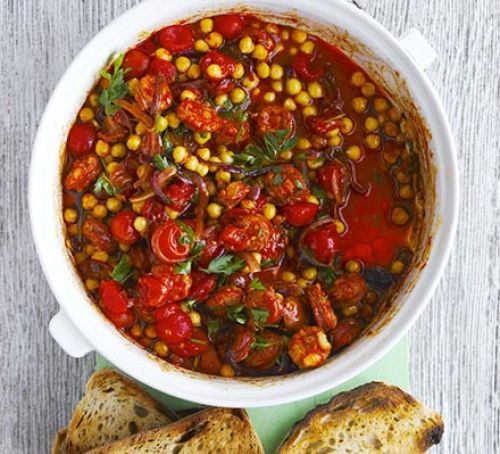
\includegraphics[height = 10cm]{ccsoup}
  \end{center}
\end{figure}

\bf{Ingredients} \normalfont \\
400g can chopped tomato \\
110g pack of chorizo sausage (unsliced) \\
140g wedge Savoy cabbage \\
sprinkling dried chilli flakes \\
410g can chickpea, drained and rinsed \\ 
1 chicken or vegetable stock cube \\
crusty bread or garlic bread, to serve \\

Put a medium pan on the heat and tip in the tomatoes, followed by a can of water. While the tomatoes are heating, quickly chop the chorizo into chunky pieces (removing any skin) and shred the cabbage. \\

Pile the chorizo and cabbage into the pan with the chilli flakes and chickpeas, then crumble in the stock cube. Stir well, cover and leave to bubble over a high heat for 6 mins or until the cabbage is just tender. Ladle into bowls and eat with crusty or garlic bread.

\section{Gulaschsuppe}
\label{gulasch}

\bf{Serves: ??} \\
\bf{Cooking Time: 1hr} \\

\bf{Ingredients} \normalfont \\
12 Zwiebeln \\
500g Rindfleisch \\ 
1 Liter Fleischbr\"{u}he  (beef stock) \\
100g Schweineschmalz  \\
1 tblsp Paprikapulver, scharf \\ 
2 tblsp Paprikapulver, edels\"{u}ss  \\
1 tsp 	Kuemmel, zerstossen  \\
\nicefrac{1}{2} tsp 	Majoran, gerebbelt \\
1 tsp 	Salz \\
2 Kartoffel(n), geschaelt und gewuerfelt \\
2 Paprikaschote(n), grün, enthäutet, in Streifen geschnitten \\
4 Tomate(n), geschaelt und gewuerfelt \\
1 Zehe/n 	Knoblauch, gepresst \\
100 ml 	Wein, rot \\
Saure Sahne (dollop for serving) \\

Die Zwiebel schaelen und in Würfel schneiden. Das Fleisch in kleine Würfel schneiden und dabei alle Sehnen und H\"{a}utchen entfernen. \\

Das Schmalz im Topf zerlassen und die Zwiebelw\"{u}rfel darin von allen Seiten goldbraun anbraten. Die Fleischw\"{u}rfel zugeben und 5 Min. unter ständigem Umwenden im Fett roesten. Das Paprikapulver, Kuemmel, Majoran und das Salz zugeben, mit der Fleischbrühe auffuellen und alles 1 Std. zugedeckt bei milder Hitze garen. \\ 

Die Kartoffelw\"{u}rfel, die Paprikastreifen und die Tomatenw\"{u}rfel mit dem Knoblauch in die Suppe rühren und weitere 25 Min. kochen lassen. Die Suppe vom Herd nehmen und den Rotwein darunter ruehren. Mit einem Klecks saurer Sahne servieren.

\section{Minestrone Suppe}
\bf{Serves: ??} \\
\bf{Cooking Time: ??} \\

\bf{Ingredients} \normalfont \\
1 mittelgrosse Zwiebel \\
1 Moehre \\
1 Stange Sellerie        \\
1-2 Knoblauchzehen \\
gehackte Petersilie \\
1 Dose Pelati, also Dosentomaten, pueriert \\
1 Suppenwuerfel, stock cube  \\
1 Dose Borlettibohnen oder rote Kidneybohnen \\
1-2 Haende Erbsen (haendevoll Erbsen, die Erbse selbst hat keine Haende) \\
2 Kartoffeln, in wuerfeln oder Oktaeder \\
Suppenpasta und Wuerstchen nach Belieben \\


Oel in einem Suppentopf erhitzen. Zwiebeln, Sellerie, Moehre und Knoblauch (alles gehackt) langsam darin anduensten.\\ 

Dann die Dose puerrierte Tomaten, Suppenwuerfel die Bohnen, Erbsen und Kartoffeln hinzugeben. Mit etwas kaltem Wasser (1-2 Tassen) auffuellen und ca 2 Stunden vor sich hin koecheln lassen. Zum Schluss Wuerstchen und Suppenpasta dazugeben. \\

Mit geriebenm Parmesan bestreuen. \\

Presto: Bon appetito

\section{\cancel{Nikki's} Favourite Soup}

\bf{Serves: ??} \\
\bf{Cooking Time: ??} \\ 

\bf{Ingredients} \normalfont \\ 
1.5 ltr chicken stock \\
100g short grain white rice \\
1 skinless, boneless chicken breast cut into matchsticks.\\
3 Tablespoons freshly squeezed lemon juice \\
3 large egg yolks \\
60g freshly grated Parmesan \\
freshly grated nutmeg to taste \\
Salt and Pepper \\
Fresh flatleaf parsley \\
 
In a large pot bring the chicken stock to the boil. Reduce heat, add the rice and simmer covered for 5 min. Add the chicken and simmer for 5 more minutes. Taste the seasoning. Meanwhile in a large bowl combine the lemon juice, egg yolks and whisk 
to blend and add half the cheese. Set aside. \\

At serving time: (the soup can be prepared several hours in advance). Add a ladleful of warm but not boiling soup to the egg mixture and whisk to blend. It is important not to use boiling soup as this will cook the egg and you will end up with scrambled egg in soup! Pour back into the pot whisking briskly until well blended. Add 
nutmeg and garnish with remaining cheese and parsley.

\section{Paprikarahm Suppe}
\begin{center}
 \it{a la Nicole aus der Markthalle} \normalfont \\
\end{center}

\bf{Ingredients} \normalfont \\
Gelbe Paprikaschoten \\
Zwiebeln \\ 
Br\"{u}he \\
Sahne \\
Schale und Saft von Zitrone (oder frisches Zitronengrass) \\
Orangenschale \\
Weisswein \\
Salz, Pfeffer, etwas Chili \\

Die Zwiebeln in Butter anschwitzen. Paprika dazugeben und weiter anschwitzen. Mit Weisswein abl\"{o}schen und dann mit der Br\"{u}he auff\"{u}llen und ca 30 min k\"{o}cheln lassen. \\

Schale und Saft der Zitrone sowie die Orangenschale dazugeben. Die Sahne hinzufügen und pürieren. Zum Schluss mit Salz, Pfeffer und Chili abschmecken. Nochmals aufkochen und evt etwas anbinden. \\

In der Markthalle wurde dies dann mit Sahneh\"{a}ubchen und einigen Streifen Safran serviert. 

\section{Tomato and Lentil Soup}
\bf{Serves: 4} \\
\bf{Cooking Time: ??} \\

\bf{Ingredients} \normalfont \\
115g red lentils \\
850ml stock \\
1 onion, peeled and chopped \\
2 carrots, peeled and chopped (optional)\\
1 $\times$ 400g can of chopped tomatoes \\
2 tsp fresh thyme \\
Salt and freshly ground black pepper \\


\it{garnish} \normalfont \\
Chopped fresh parsley \\
Cro\^{u}tons \\

Place all the ingredients into a saucepan and bring to the boil on the hob. Simmer for about 45--60 minutes. Once cooked you may liquidise if prefered. Adjust the seasoning and garnish with the chopped fresh parsley and cro\^{u}tons. We then normally also add a splash of white wine or sherry vinegar. 





\part{Main Courses}
\setcounter{chapter}{0}
\chapter{Beef}

\section{Dad's Bhoona Gosht (either lamb or beef)}
\hyperref[bhoona]{see here}

\section{Gulaschsuppe}
\hyperref[gulasch]{see here}

\section{Joe's Beef and Mushroom Pie}
\bf{Serves: 4} \\
\bf{Cooking Time: ??} \\
See next page
\begin{figure}[h!]
  \begin{center}
  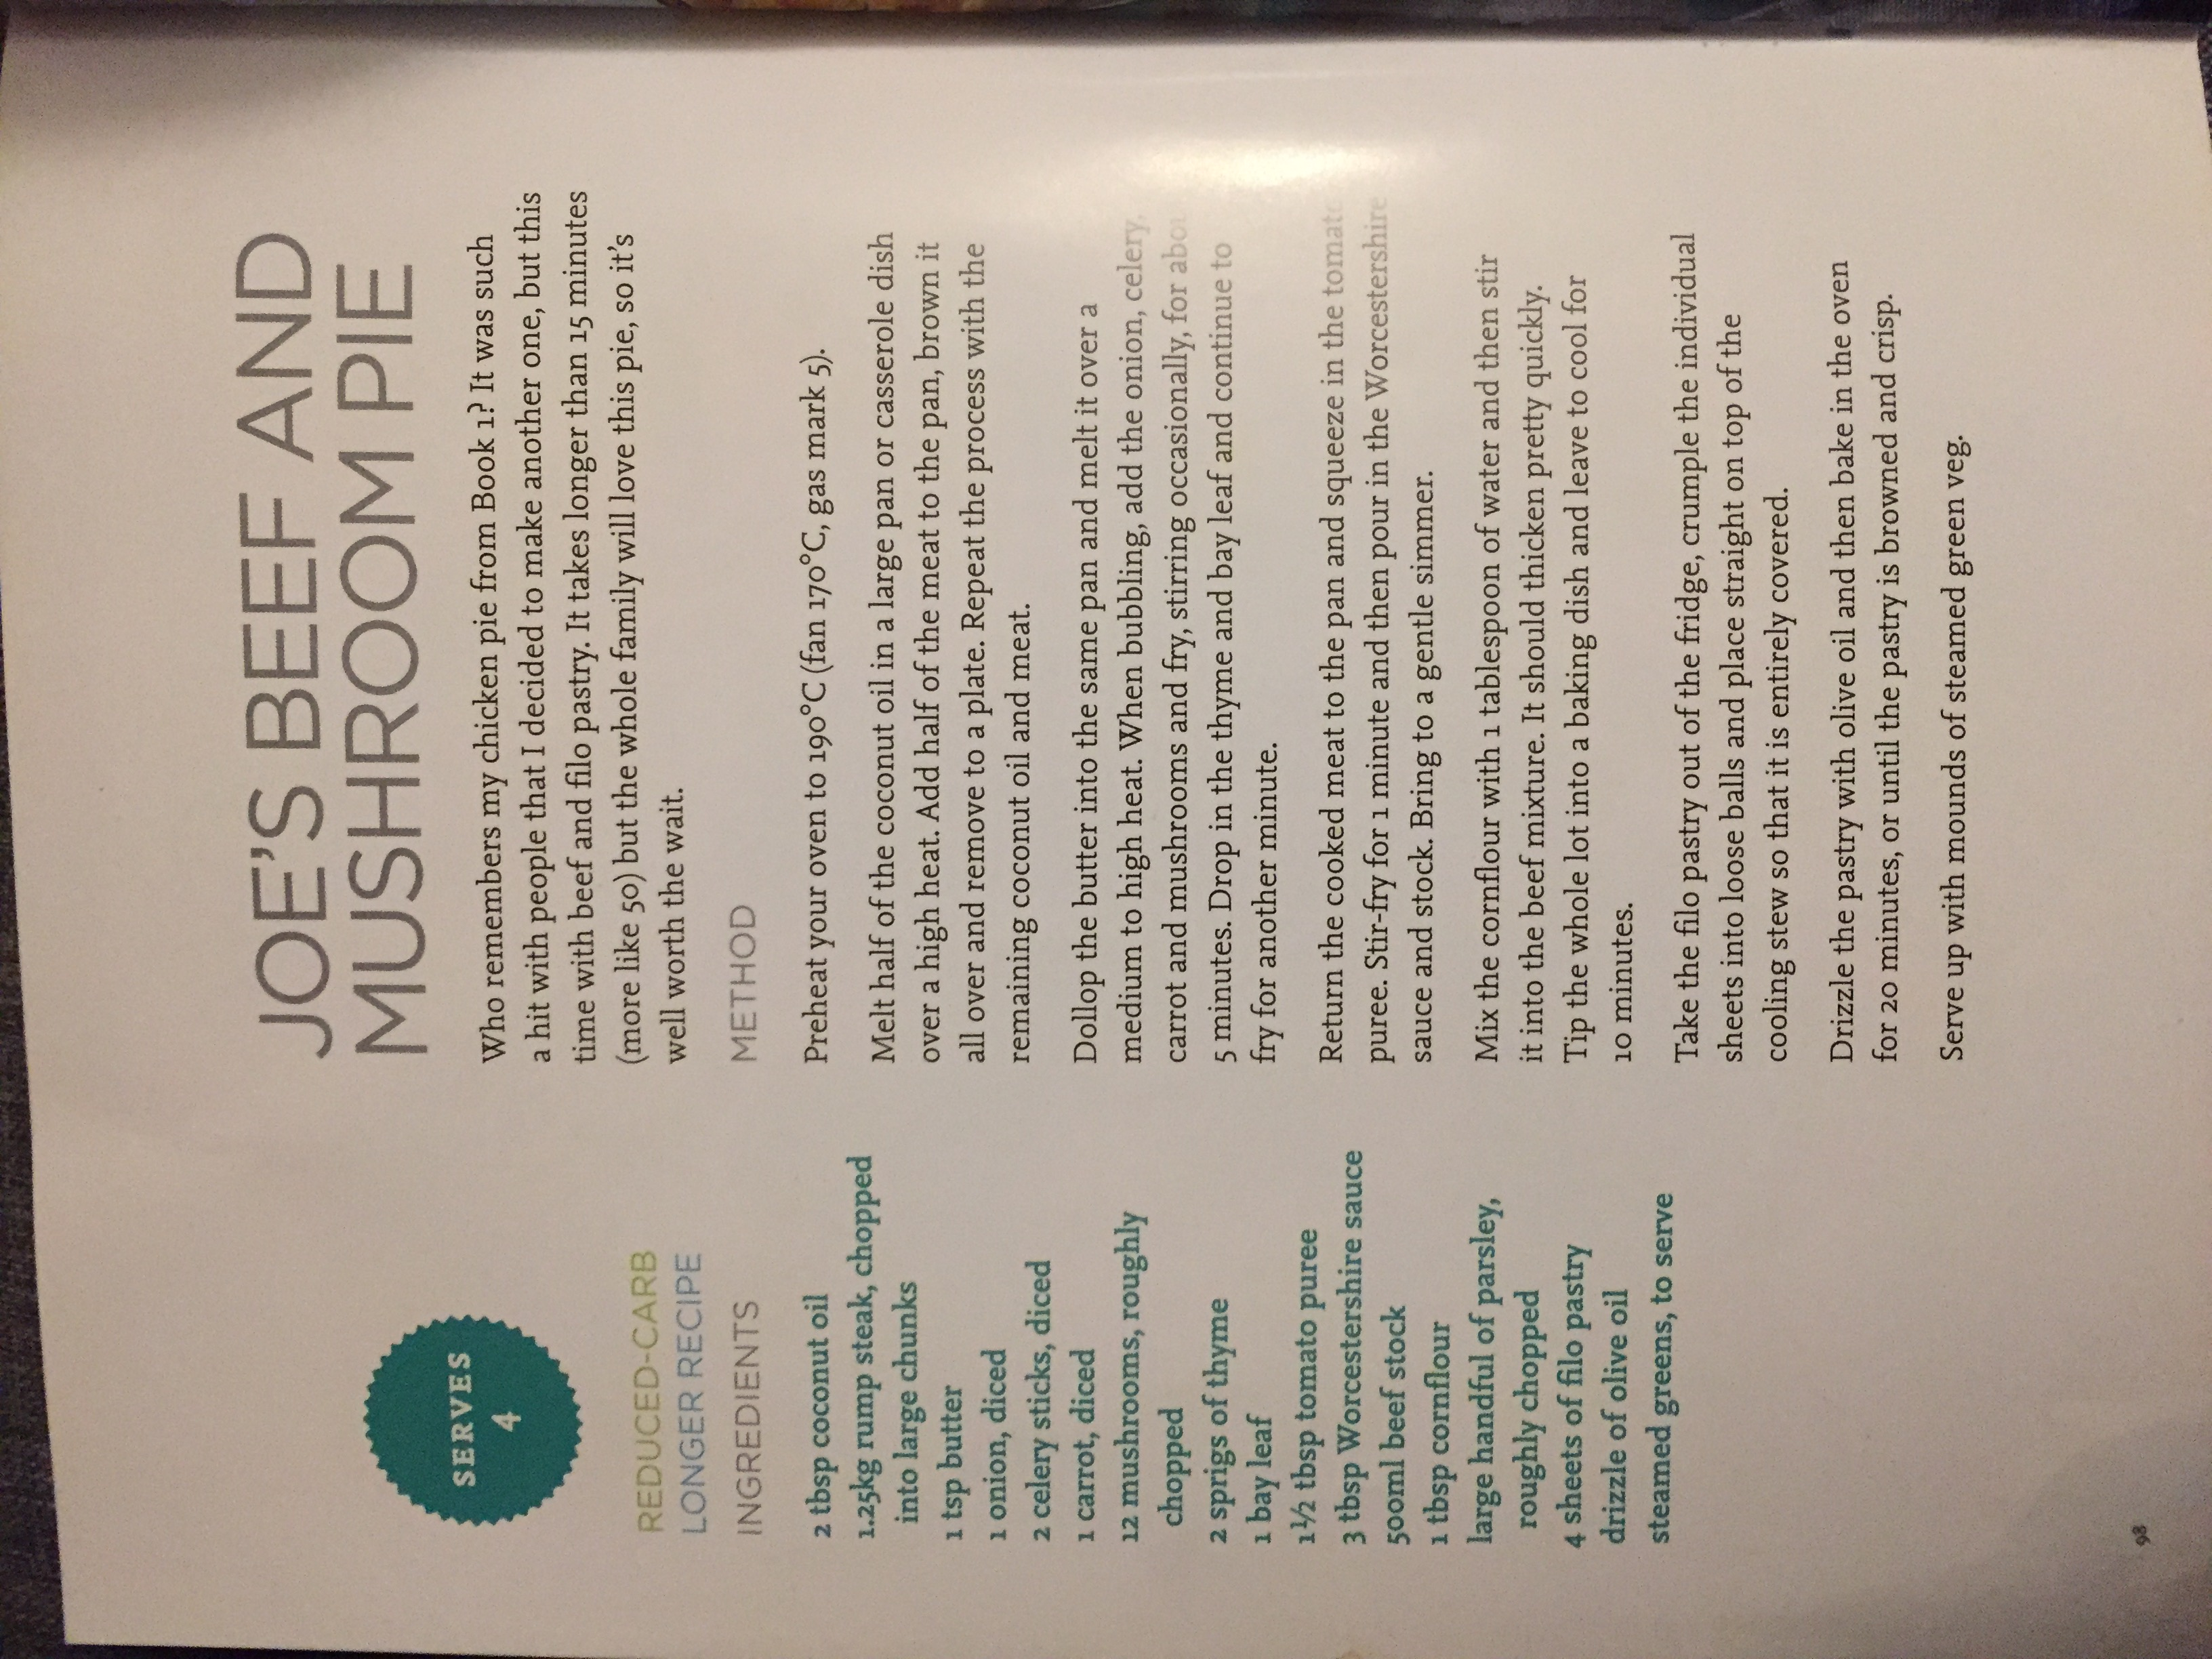
\includegraphics[height = 14cm, angle=270]{BeefPie}
  \end{center}
\end{figure}

\section{Smoked beets with grilled steak and a cottage cheese dressing}
\bf{Serves: 2} \\
\bf{Cooking Time: ??} \\

\bf{Ingredients} \normalfont \\ 
8 small beets, tops trimmed \\
Small bunch of fresh rosemary, leaves picked \\
1 TBSP red wine vinegar \\
Several glugs of extra virgin olive oil \\
Sea salt, freshly ground pepper to taste \\
Small bunch of fresh flat-leaf parsley, leaves picked and roughly chopped \\
Small bunch of fresh tarragon or basil, leaves picked and roughly chopped \\
4 four-ounce fillet steaks \\

\textit{For the dressing} \\
4 heaping TBSP cottage cheese \\
½ lemon (juice and grated zest) \\
A few glugs of extra virgin olive oil \\
A few sprigs of fresh thyme, leaves picked \\

Preheat oven to 400 degrees. Place trimmed beets on a large strip of foil, top with rosemary leaves. Roll up, folding edges and twisting the ends together. Pop it in the oven for 1.5 hours. Unwrap and let the beets cool a bit. Once cool enough to handle, peel and discard skin. Cut into irregular chunks and place in bowl. Top with vinegar and 3 or so TBSPs of extra virgin olive oil, a hearty shake or five of sea salt and pepper and half of the parsley and tarragon or basil. Toss, adjust seasoning to taste. \\

Put cottage cheese into a bowl, add lemon juice and zest. Stir in two glugs of olive oil, add the thyme, a generous dash of salt and pepper and fold together so that the lemon and oil appear to marble through the cottage cheese. Taste and adjust seasoning. \\

Rub some of the dressing on steaks. Throw into pre-heated (medium-high) sauté skillet and cook to your liking. (Mine were nicely browned but on the rare side — I gave them about two minutes a side). Remove from pan and let them rest. \\

Divide the beets between two plates, top with the steaks, dressing, throw on the extra herbs and dig in.

\section{Thai Beef Mango Salad}
\bf{Serves: 2} \\
\bf{Preparation: 30 minutes, Cooking Time: 10 minutes} \\

\bf{Ingredients} \normalfont \\
2 beef frying steaks \\
1 tbsp vegetable oil \\
1 tbsp soy sauce \\
2 small carrots \\
5 spring onions \\
1 ripe mango \\
2 baby gem lettuces or 1 small lettuce \\
handful of salted peanuts (about 40g), optional \\

\textit{For the dressing} \\
1 garlic clove \\
1 lime, juice only \\
1 tbsp caster sugar \\
1 tsp chilli flakes \\

Put the steaks in a shallow bowl. Pour on the oil and soy sauce and rub them into the meat so it's coated all over. Set aside to marinate while you prepare the vegetables. Peel the carrots then use the peeler to make thin ribbons. Separate the lettuce leaves, wash the leaves and drain in a colander. Finely slice the spring onions then peel, stone and thinly slice the mango. Combine the vegetables in a large bowl. \\

Heat a large frying pan over a high heat, add the steaks and cook for 1 minute on each side for medium rare or cook for an extra minute on each side for medium. Remove the steaks from the pan and transfer to a plate to rest. \\

While the steaks are resting, prepare the dressing. Peel and grate the garlic then put it into a bowl with the lime juice, sugar and chilli flakes and stir them together. Pour the dressing over the prepared vegetables and add the peanuts. Slice the beef thinly, add to the bowl along with any resting juices and toss to combine. Serve immediately.



\section{World's Best Chilli Con Carne}
\bf{Serves: ??} \\
\bf{Cooking Time: ??} \\

\bf{Ingredients} \normalfont \\ 
800g lean diced beef \\
125g Pancetta (cubed bacon) \\
1 tblsp olive oil \\
2 onions, peeled and chopped \\
2 Cloves Garlic, peeled and crushed \\
2 large red chillies, deseeded and chopped \\
2-3 tsp of hot chilli powder \\ 
1 can chopped tomatoes (400g) \\
1 rounded tblsp Tomato Puree \\
450ml Beef Stock \\
1 can red kidney beans (400g) \\
1 red pepper, deseeded and diced \\
\it{secret ingredient}: \normalfont  25g of dark chocolate\\
 
Heat half of the olive oil in a large frying pan over high heat and brown the beef in batches. Place in a flameproof casserole dish and set aside. Heat remaining oil in pan and add the diced Pancetta. Cook over medium heat until pancetta just beginning to colour. Add Onions. Cook for 3-4 min until tender, add crushed garlic, chopped chilli and chilli powder. Cook for a further minute and then add stock (dissolved cube is fine). Bring to the boil and stir with wooden spoon. Pour contents into flameproof casserole add the tomatoes, tomato puree and seasoning. Bring to boil, reduce heat to very gentle simmer, cover and cook for about 1 hr 30 min or until meat is tender (Alternatively put into oven set to 140-160 degree. Rayburn is ideal!). \\

Taste and check the seasoning. Drain and rinse the kidney beans and add to the chilli along with the red pepper. Continue to cook for further 5-10 min until veg are cooked. And now the \it{secret ingredient}: \normalfont 25 g of dark chocolate. I know, sounds crazy but you will notice a nice silky smooth difference. \\

Serve with Guacamole (see \hyperref[guacamole]{guacamole}), Tortilla chips, rice and sour cream.

\chapter{Chicken}

\section{Chicken and Broccoli Bake}

\bf{Serves: 2} \\
\bf{Cooking Time: 45 minutes} \\
\bf{Rating: 7/10} \\

\bf{Ingredients} \normalfont \\
295g tin of condensed chicken soup \\
6 $\times$ 15ml spoon of mayonaise \\
210ml milk \\
1 head of broccoli \\
450g potatoes; peeled, skinned and par-boiled \\
350g chicken, cooked, diced \\
175g Red Leicester cheese \\

Preheat the oven to 200$^{\circ}$C. Mix the soup, mayo, milk and seasoning. Then pour half the mixture into a casserole dish and then arrange the broccoli evenly over soup, add chicken and finely sliced potatoes. Then add remaining mixture and cook for 30 minutes. Then sprinkle over the cheese and cook for another 15 minutes. 

\section{Crispy and Sticky Chicken Thighs with Squashed New Potatoes 
and Tomatoes}


\bf{Serves: 4} \\
\bf{Cooking Time: ??} \\

\bf{Ingredients} \normalfont \\
800g new potatoes \\
Pinch of sea salt and black pepper \\
12 boned chicken thighs, skins on, preferably free-range or organic \\
Splash of olive oil\\
600g cherry tomatoes \\
Bunch of fresh oregano \\
Splash of red wine vinegar \\

This is a simple tray baked dish, the food you absolutely love to eat! You can increase the quantities and you can feed an army. Or put 2 trays on so the proportions are preserved. While it is in the oven you can sip a glass of wine and put the world to right.\\

Scrub the potatoes and put them in a large saucepan and cook until nearly done. While the Buntattas are boiling, preheat the oven to 200$^{\circ}$C. Cut each de-boned chicken thigh into 3 strips and place in a bowl. Rub the meat all over with olive oil, salt and pepper. Give it a good toss. Heat a large frying pan, big enough to hold all 
chicken bits in a single layer. You may have to do that in batches if the pan not big enough. Fry the pieces skin side down over a high heat for 10 minutes or so until almost cooked. Remove with a slotted spoon to an ovenproof pan or dish. \\

If you feel like a domestic goddess skin the tomatoes. (Prick with a sharp knife and cover with boiling water. Leave for a minute or so. Drain. Once cool enough to handle pinch of their skin.) I never do this. Drain the potatoes in a colander and gently crush them down. \\

Bash up most of the oregano leaves with a pinch of salt in a pestle and mortar. Add 4 tablespoons of olive oil and a good splash of red wine vinegar and some black pepper. (an empty screw top jar will serve as a shaker). Add to the chicken, tomatoes and potatoes. Scatter remaining oregano leaves and toss everything together. Bake for 40 
min in the pre-heated oven until lovely and golden. \\

Serve with simple salad and a glass of white wine.

\section{Devilled Chicken Legs}


\bf{Serves: 4} \\
\bf{Cooking Time: ??} \\

\bf{Ingredients} \normalfont \\
8 chicken drumsticks \\
Sunflower Oil \\

\it{For the sauce}: \normalfont \\
1 tablespoon of clear honey \\
2 tablespoons of sunflower oil \\
1 tablespoon of Worchester Sauce \\
a generous pinch of cayenne pepper \\
1 tablespoon of Dijon mustard \\
Half teaspoon salt \\

This devilling sauce is perfect for smearing over chicken that is about to be grilled or barbecued. The anointed drumsticks can also be cooked in the oven. \\

Pre-heat the oven to 200$^{\circ}$C. Mix together the sauce ingredients and brush or smear all over the drumsticks. Oven: Arrange drumsticks on a lightly oiled shallow baking tray then place in the oven for 30 min, turning occasionally, until well browned and cooked right through to the bone. Serve hot or cold.\\

Grill: Pre-heat grill thoroughly. Line grill pan with silver foil, then arrange the drumsticks on the rack and grill, about 10 cm from the heat, turning frequently until dark brown and cooked through to the bone. Brush with any leftover sauce as they cook.

\section{Devilled Chicken Pie}


\bf{Serves: 4} \\
\bf{Cooking Time: ??} \\

\bf{Ingredients} \normalfont \\
1kg chicken breast, skinless and boneless cut into 4 cm cubes, 
although I like to make it with leg meat as it is far juicier. \\
1 tsp dried rosemary and thyme, crushed \\
Salt and pepper \\
2 tsp olive oil \\
2 tblsp Worcester sauce \\
6 anchovy fillets, pounded to a paste \\
300ml double cream \\
1 tsp paprika \\

\it{For the Mash: }\normalfont \\
4 large potatoes \\
150ml milk \\
100g butter \\

Preheat oven to 220$^{\circ}$C. Coat the chicken cubes in herbs and seasoning. Heat oil in frying pan and seal the chicken. It does not have to be cooked right through at this point. Mix Worcester sauce and anchovies in a bowl until well blended. Pour in the cream and sprinkle with Paprika. Now make the mash. Once tatties cooked mash with the butter and milk to end up with a fairly soft mash. Add some salt.

Fill a pie dish with the chicken and anchovy sauce mixed well together. Top with the mash. If you feel artistic you can use a fork to decorate the surface. Pop in the oven and bake for 30 min until golden.

Serve with roast vegetables such as parsnip, sweet potatoes, carrots and butternut squash. Today we just served it with some green salad.

\section{French Roast Chicken}

\bf{Serves: ??} \\
\bf{Preparation Time: 15  minutes}
\bf{Cooking Time: 1.25 hours} \\ 

\bf{Ingredients} \normalfont \\
15g of butter \\
1tbls vegetable oil \\
1.6kg whole chicken \\
pinch of salt \\
ground black pepper \\
2 cloves of garlic \\
12 rosemary sprigs \\
12 thyme sprigs \\
150ml chicken stock \\
slug of white whine \\
3tbls double cream \\

Preheat the oven to 200$^\circ$C. Melt the butter with the oil in a large frying-pan, add the chicken and cook, turning constantly, for 5 minutes or until golden brown. Transfer to a medium sized casserole dish. Reserve the cooking juices in the frying-pan. \\

Season the chicken with salt and pepper. Tuck the cloves of garlic and about 4 sprigs of both rosemary and thyme under the legs. Pour 50ml of the chicken stock over the chicken, cover and cook for 45 minutes. Uncover and cook for another 15 minutes. \\

Remove from the oven, transfer the chicken to a warmed serving dish and keep warm in a low oven while you prepare the sauce. \\

Strain the juices from the casserole into the frying-pan. Pour in the reserved stock and bring to the boil, stirring constantly. Continue boiling until it is reduced by half then allow to cool slightly before stirring in the cream. Serve the chicken surrounded by the remaining rosemary and thyme with the sauce. \\

\section{Jaime Oliver's Chicken \& Leak Stew}

\textit{We tried a \hyperref[vegversion]{veggie version} using quorn which also worked very well. \\ }

\textbf{Serves: 4} \\
\textbf{Cooking Time: ?} \\ 

\textbf{Ingredients}\\ 
2 tblsp extra-virgin olive oil \\
2 medium leeks, white and tender green parts only, thinly sliced \\
200-300g cremini mushrooms, thinly sliced \\
Salt and freshly ground pepper \\
1 pound skinless, boneless chicken breast halves, cut into 2-inch pieces \\
All-purpose flour, for dusting \\
1 1/2 cups chicken stock or low-sodium broth \\
1 tblsp chopped thyme \\ 
2 tblsp sour cream \\
2 tsp Dijon mustard \\

\textit{Serve with garlic bread and rice/potatoes} \\

In a pan, heat 1 tablespoon of the oil. Add the leeks and cook over moderate heat, stirring, until softened, about 7 minutes. Add the mushrooms and season with salt and pepper. Cover and cook, stirring, until the mushrooms are tender, about 4 minutes. Scrape the leeks and mushrooms onto a plate. \\

Season the chicken with salt and pepper and lightly dust with flour, shaking off any excess. Heat the remaining 1 tablespoon of oil in the skillet. Add the chicken and cook over moderate heat until golden brown, about 2 minutes per side. Add the chicken stock and thyme and simmer over moderate heat until the chicken is just cooked through, about 1 minute. Using a slotted spoon, transfer the chicken to the plate with the vegetables. \\

Simmer the stock over moderately high heat until reduced by half, about 2 minutes. Return the chicken, leeks and mushrooms to the skillet and simmer over low heat until warmed through, about 1 minute.  \\

In a small bowl, blend the sour cream with the mustard (Alistiar says 2tsp is too much apparently but I liked it) and stir into the stew. Remove the skillet from the heat. Season the stew with salt and pepper and serve. Serve With new potatoes or steamed rice and garlic bread.



\section{Satay Chicken Thighs}

\textbf{Serves: 4--6} \\
\textbf{Cooking Time: 55 minutes} \\ 

\textbf{Ingredients}\\ 
12 boneless skinless chicken thighs \\
2 tbsp diced garlic \\
2 tbsp rice wine vinegar \\
2 white onions diced \\
pinch of corriander \\
60ml of Hoisin sauce \\
60ml soy sauce \\
2 tbsp oil \\
2 tbsp peanut butter \\
1 tsp crushed red pepper flakes or chilli powder \\

Combine ingredients and marinate chicken thighs at least overnight (not really neccessary, just do it for a bit). Preheat oven to 350$^{\circ}$C and cook for 20 minutes then flip the thighs and cook for a further 25 minutes. 

\section{Thai Green Chicken Curry}

\bf{Serves: 4} \\
\bf{Cooking Time: 30--40 minutes} \\ 
\bf{Rating: \mystar  \mystar  \mystar  \mystar  \mystar} \\ 

\bf{Ingredients} \normalfont \\ 
225g sweet potatoes (or new potatoes), cut into chunks \\
100g green beans, trimmed and halved \\
1 green pepper sliced \\
1 tbsp vegetable or sunflower oil \\
1 garlic clove, chopped \\
1 rounded tbsp or 4 tbsp Thai green curry paste \\
400ml can coconut milk \\
2 tbsp Thai fish sauce \\
1 tbsp caster sugar \\
450g boneless skinless chicken (breasts or thighs), cut into bite-size pieces \\
2 fresh kaffir lime leaves finely shredded, or 3 wide strips lime zest, plus extra to garnish \\
good handful of basil leaves \\
boiled rice, to serve \\
dash of soy sauce \\

Either microwave the sweet potatoes for 4 minutes or put the potatoes in a pan of boiling water and cook for 5 minutes. Throw in the beans and cook for a further 3 minutes, by which time both should be just tender but not too soft. Drain and put to one side. \\

In a wok or large frying pan, heat the oil until very hot, then drop in the garlic and cook until golden, this should take only a few seconds. Don’t let it go very dark or it will spoil the taste. Spoon in the curry paste and stir it around for a few seconds to begin to cook the spices and release all the flavours. Next, pour in the coconut milk and let it come to a bubble. \\

Stir in the fish sauce and sugar, then the pieces of chicken. After 4 minutes throw in the pepper and beans (if not boiled with the potatoes). Turn the heat down to a simmer and cook, covered, for about 4 minutes until the chicken is cooked. Tip in the potatoes and beans and let them warm through in the hot coconut milk, then add a lovely citrussy flavour by stirring in the shredded lime leaves (or lime zest). The basil leaves go in next, but only leave them briefly on the heat or they will quickly lose their brightness. Scatter with the lime garnish and serve immediately with boiled rice.

\chapter{Seafood}

\section{Chilli prawn linguine}

\bf{Serves: 4} \\
\bf{Cooking Time: 30 minutes} \\
\bf{Rating: 9/10} \\

\bf{Ingredients} \normalfont \\

280g linguine pasta \\
200g sugar snap peas, trimmed \\
2 tbsp olive oil \\
2 large garlic cloves, finely chopped \\
1 large red chilli, deseeded and finely chopped \\
24 raw king prawns, peeled \\
12 cherry tomatoes, halved \\
a handful of fresh basil leaves \\
mixed salad leaves and crusty white bread, to serve \\

\textit{For the lime dressing \\}
2 tbsp virtually fat-free fromage frais \\
grated zest and juice of 2 limes \\
2 tsp golden caster sugar \\

To make the dressing, mix 2 tbsp fromage frais, the grated zest and juice of 2 limes and 2 tsp golden caster sugar in a small bowl and season with salt and pepper. Set aside.\\

Cook 280g linguine pasta according to the packet instructions. Add 200g trimmed sugar snap peas for the last minute or so of cooking time.\\

Meanwhile, heat 2 tbsp olive oil in a wok or big frying pan, toss in 2 finely chopped large garlic cloves and 1 deseeded and finely chopped large red chilli and cook over a fairly gentle heat for about 30 seconds without letting the garlic brown.\\

Tip in 24 peeled raw king prawns and cook over a high heat, stirring frequently, for about 3 minutes until they turn pink.
Add 12 halved cherry tomatoes and cook, stirring occasionally, for 3 minutes until they just start to soften. \\

Drain the linguine pasta and sugar snap peas well, then toss into the prawn mixture.\\

Tear in a handful of basil leaves, stir, and season with salt and pepper.\\

Serve with mixed salad leaves drizzled with the lime dressing, and warm crusty white bread.


\section{Creamy Prawn Curry}

\bf{Serves: 4} \\
\bf{Cooking Time: ??} \\
\bf{Rating: 8/10} \\

\bf{Ingredients} \normalfont \\

1 tbsp sunflower oil \\
2 medium onions, finely chopped \\
4 garlic cloves, finely sliced \\
20g chunk of fresh root ginger, peeled and finely chopped \\
3 tbsp Korma curry paste (we used tikka masala which was also good) \\
500ml cold water \\
2 tbsp double or single cream (except loads more than this)\\
2 tsp caster sugar \\
400g peeled raw tiger prawns, deveined if necessary and thawed if frozen \\
20g bunch of fresh coriander, leaves roughly chopped \\
flaked sea salt \\


Heat the oil in a medium non-stick saucepan or saute pan and stir in the onions, garlic and ginger. Cover the pan with a lid and cook the onions and garlic over a medium heat for 10 minutes until pale golden brown, stirring occasionally. \\

Remove the lid and stir in the curry paste. Cook for a further minute, while stirring, then add the water and bring to the boil. Lower the heat slightly and simmer for 8–10 minutes, uncovered, until the liquid has reduced by half and the onions are very soft. \\

Remove the pan from the heat and, using a stick blender, blitz to a smooth sauce. Stir in the cream and sugar, season with a little salt and put the pan back on the heat. \\

Add the prawns to the pan, bring to a simmer and cook for 3–4 minutes, stirring, until the prawns are completely pink and beginning to curl. \\

Sprinkle the fresh coriander over the top, stir well and serve the korma immediately with a small portion of rice. \\

\section{Cullen Skink}
1 tbsp olive or vegetable oil \\
1 leek, well-rinsed, chopped \\
and cut into rough 2cm cubes \\
1 litre fish stock \\
200g waxy potatoes, peeled and cut into roughly 2cm cubes \\
300g undyed smoked haddock fillet 1 bay leaf \\
freshly ground pepper \\
2 tbsp whipping cream \\
Chives, roughly chopped \\

Warm the oil in a pan. Add the chopped leek, cover and gently cook for a few minutes until soft. Add the stock, bay leaf, potato and haddock. Season lightly with black pepper. Bring to the boil and simmer for 15 minutes.\\

Remove the haddock from the pan with a slotted spoon. When the fish is cool enough to handle, remove any skin and bones, then flake the haddock back into the pan. \\

Blend a ladle full of the soup in a liquidizer and return to the pan. Stir in the double cream and simmer for another 2-3 minutes. Add more black pepper if necessary, then sprinkle with the chopped chives and serve.Serve with chunks of fresh wholemeal or granary bread. \\

\section{Hot Smoked Salmon with Avocado Salsa}

250g hot smoked salmon, flaked into large pieces \\

\textbf{For the Lobster Oil } \\
175g lobster or langoustine shells 350ml sunflower oil \\
1 tiny piece of broken star anise 3 white peppercorns \\ 
5cm piece carrot, peeled and diced 2 shallots, diced \\
5cm piece celery, diced \\
2 cloves of garlic \\
15g mixed herbs (such as parsley, thyme \& tarragon) 1/2 tsp tomato puree \\
50ml dry white wine \\

\textbf{For the Salsa } \\
1 large ripe hass avocado \\
2 ripe plum tomatoes, peeled, \\
seeded and chopped into 1cm dice \\
1/4 red onion, finely chopped \\
1 red chilli, seeded and finely chopped 1 tbsp Japanese pickled ginger, finely chopped (optional) \\
3 tbsp fresh coriander, chopped \\
2 tsp Thai fish sauce \\
Juice and zest of a lime \\
Salt \& freshly ground black pepper \\
A squeeze of lemon juice \\

Crush the shells and drain away any liquid. Heat 4 tbsp of the oil in a pan, add the shells, star anise and white peppercorns and fry over a medium heat for 15 minutes, stirring every now and then. Add all the remaining ingredients, except the oil, and cook until the wine has evaporated. Add the rest of the oil and leave to simmer for 45 minutes. Remove from the heat and leave to stand for 24 hours. Strain through a muslin-lined sieve, transfer to a bottle and seal. This will keep in the fridge for about a month. \\

To make the salsa, halve the avocado and remove the stone. Halve again and remove the skin before chopping it into 1cm chunks. Place in a mixing bowl and add the chilli, onion, coriander, pickled ginger if using, tomato, Thai fish sauce, a pinch of salt and freshly ground black pepper and the lime zest and juice. Mix well and leave at room temperature for about 10 minutes for the flavours to develop. \\ 

To serve, set a 7.5cm biscuit cutter or food ring in the centre of a plate. flake the salmon, and using about 75g per ring, press into the base of each ring, banking it up the sides of the ring so that it will hold. Spoon the salsa on top of the salmon and press down lightly. Remove the ring carefully and garnish with a small handful of slightly dressed salad leaves piled on top. Drizzle round the lobster oil. \\


\section{Scallops and Chorizo}
\label{scallopsandchorizo}
\textbf{Serves: 2} \\
\textbf{Preparation time: 30 minutes, Cooking Time: 10--30 minutes} \\

\bf{Ingredients} \normalfont \\
3 fresh chorizo sausages, sliced into rounds the thickness of a pound coin \\
4 spring onions, trimmed and sliced \\
2 red chillies, thickly sliced \\
24 scallops, cleaned (with 6 shells reserved and cleaned if you can get them) \\
2 tbsp runny honey \\

Heat a heavy griddle pan over a high heat. Fry the chorizo until it is browned and some of the juices are running in the pan. Add the spring onion and chilli and fry for 2-3 minutes. Add the scallops and fry for 2-3 minutes on either side or until cooked through. Drizzle over the runny honey and stir to coat. Divide the scallops and chorizo among the six scallop shells and serve.

\section{Teriyaki Salmon}
\bf{Serves: 2} \\
\bf{Cooking Time: 30 minutes} \\

\bf{Ingredients} \normalfont \\
2 salmon fillets \\
4-5 tbsp dark soy sauce \\
1 lime, zest and juice \\
1 small chilli \\
2 tbsp maple syrup (can replace with honey and works just as well)\\
1 fat garlic clove, finely chopped \\
1 chunk of ginger, finely chopped \\
1 sheet of egg noodles \\
1 tbsp sesame oil \\
extra lime juice \\

Heat some olive oil in a pan and fry the ginger, garlic and chopped chilli. Add the zest and juice of the lime and pour in the soy sauce. Add the maple syrup and cook for 1 minute or until reduced and sticky. Meanwhile, pan-fry the two pieces of salmon for 2 minutes each side in a hot griddle pan. \\

When the sauce is reduced add the salmon to the teriyaki sauce frying pan. Cook and drain the noodles, adding the sesame oil, seasoning and a squeeze of lime. Serve the salmon on a bed of noodles.

\section{Thai Fish Curry}
\bf{Serves: } \\
\bf{Cooking Time: } \\

\bf{Ingredients} \normalfont \\
2 tbsp sunflower or groundnut oil \\
400ml tin of coconut milk \\
200ml fish stock or water \\
2 tbsp Thai fish sauce (nam pla) \\
2 tsp sugar \\
125g French beans \\
100g spring onions \\
500g firm fish fillets, such as pollack, gurnard or grey mullet, skinned \\
300g fresh crabmeat - a mix of white and brown, or all white if you prefer
A handful of coriander, Thai basil or ordinary basil leaves, roughly torn \\

\bf{For the curry paste} - \it{Alternatively just buy some curry paste} \normalfont \\
2-6 small green chillies, according to heat, deseeded if you like \\
3-4 small shallots or 1 small onion, chopped \\
100g fresh ginger, chopped \\
4 garlic cloves, peeled \\
2 tbsp galangal paste (optional) \\
3 lemongrass stalks, tough outer layers removed, finely sliced \\
2 tsp ground coriander \\
2 tsp ground cumin \\
Juice and grated zest of 1 lime \\
4 kaffir lime leaves, chopped (optional) \\
1 tsp Thai shrimp paste \\
1 tsp sea salt \\

Put all the curry paste ingredients into a food processor or blender and whiz to a fairly smooth paste, adding a tablespoon of water to help it along if necessary. \\

Heat the oil in a heavy-based saucepan, then scrape in the curry paste. Fry over a low-medium heat for 3-4 minutes, stirring often, without letting it colour. Add the coconut milk, stock or water, fish sauce and sugar. Bring to a gentle simmer and cook, uncovered, for 20-25 minutes. \\

Meanwhile, cut the French beans into 2-3cm lengths and slice the spring onions on the diagonal. Add these to the curry sauce and cook for 5 minutes. \\

Cut the fish fillets into large bite-sized pieces. Add these to the pan, cover with a lid and simmer gently for 2-3 minutes, until the fish is just cooked. Stir in the crabmeat and heat through gently for another minute. \\

Serve in deep bowls, scattered with the coriander or basil and accompanied by boiled rice. \\

\chapter{Lamb}

\section{Dad's Bhoona Gosht (either lamb or beef)}
\label{bhoona}
\bf{Serves: ??} \\
\bf{Cooking Time: ??} \\

\bf{Ingredients} \normalfont \\
1.5 pounds of lean meat \\
1 inch of root ginger \\
2 cloves of garlic \\
4 oz. of tomatoes \\
1 stick of cinnamon \\
cardamom, optional \\
2 bay leaves \\
3--4 oz. of yogurt \\
2 big onions chopped or crushed \\
salt, to taste \\
1 tbsp of coriander powder \\
1/2 tsp of turmeric powder \\
1/2 tsp of chilli powder \\
1/2 tsp of garam masala \\
chopped coriander to garnish \\

Chop onion, ginger, and green chilli finely. Heat the ghee or cooking oil add crushed cardamom, bay leaf and cinnamon. Fry these for a few minutes and then add the onions, garlic and chilli. Fry these for 2--3 minutes, now add meat and brown them. Add turmeric, coriander, salt, chilli powder, yogurt, tomatoes and mix well. Cover with a light fitted lid and cook until the meat is tender. Take the lid off and increase the heat and stir fry until all the moisture is evaporated. Sprinkle with garam masala and coriander leaves. Serve with boiled rice and naan bread. 

\chapter{Pork}

\section{Chorizo and Chickpea Soup}
\textbf{Serves: 3 lunch portions, when served with bread} \\
\textbf{Cooking Time: 15 minutes} \\ 

\textbf{Ingredients} \\
400g can chopped tomato \\
110g pack of chorizo (half a sausage) \\
140g wedge Savoy cabbage \\
sprinkling dried chilli flakes \\
410g can chickpea, drained and rinsed \\
1 chicken or vegetable stock cube \\
crusty bread or garlic bread, to serve \\
 
Put a medium pan on the heat and tip in the tomatoes, followed by a can of water. While the tomatoes are heating, quickly chop the chorizo into chunky pieces (removing any skin) and shred the cabbage. \\

Pile the chorizo and cabbage into the pan with the chilli flakes and chickpeas, then crumble in the stock cube. Stir well, cover and leave to bubble over a high heat for 6 mins or until the cabbage is just tender. Ladle into bowls and eat with crusty or garlic bread.

\section{Chorizo Hotpot}

\bf{Serves: 4} \\
\bf{Cooking Time: ??} \\ 

\bf{Ingredients} \normalfont \\
1 onion \\
Half a chorizo sausage \\
3 cloves of garlic \\
2 bayleaves \\
A splash of sherry \\ 
4 large Potatoes \\
Handful of french beans \\

Fry the onions for 5 minutes. Then add chorizo, bayleaves and sherry and then the dices potatoes. Add just enough water to cover. \\

This is the recipe as such. But we found it even better with some french beans thrown in towards the end to make a complete meal in itself.

\section{Courgette Carbonara}

\bf{Serves: ??} \\
\bf{Cooking Time: ??} \\

\bf{Ingredients} \normalfont \\
sea salt \\
freshly ground black pepper \\
6 medium courgettes , mix of green and yellow if available \\
500 g penne \\
4 large free-range egg yolks \\
100 ml single cream \\
1 small handful Parmesan cheese , freshly grated \\
olive oil \\
6 slices higher-welfare back bacon , cut into chunky lardons \\
1 small bunch fresh thyme , leaves picked and chopped, flowers reserved (if you can get hold of flowering thyme) \\
a few courgette flowers , optional \\

Before you start cooking, it’s important to get yourself a very large pan, or use a high-sided roasting tray so you can give the pasta a good toss. Put a large pan of salted water on to boil. Halve and then quarter any larger courgettes lengthways. Cut out and discard any fluffy middle bits, and slice the courgettes at an angle into pieces roughly the same size and shape as the penne. Smaller courgettes can simply be sliced finely. Your water will now be boiling, so add the penne to the pan and cook according to the packet instructions. \\

To make your creamy carbonara sauce, put the egg yolks into a bowl, add the cream and half the Parmesan, and mix together with a fork. Season lightly and put to one side. \\

Heat a very large frying pan (a 35cm one is a good start – every house should have one!), add a good splash of olive oil and fry the pancetta or bacon until dark brown and crisp. Add the courgette slices and 2 big pinches of black pepper, not just to season but to give it a bit of a kick. Sprinkle in the thyme leaves, give everything a stir, so the courgettes become coated with all the lovely bacon-flavoured oil, and fry until they start to turn lightly golden and have softened slightly. \\

It’s very important to get this next bit right or your carbonara could end up ruined. You need to work quickly. When the pasta is cooked, drain it, reserving a little of the cooking water. Immediately, toss the pasta in the pan with the courgettes, bacon and lovely flavours, then remove from the heat and add a ladleful of the reserved cooking water and your creamy sauce. Stir together quickly. (No more cooking now, otherwise you’ll scramble the eggs.) \\

Get everyone around the table, ready to eat straight away. While you’re tossing the pasta and sauce, sprinkle in the rest of the Parmesan and a little more of the cooking water if needed, to give you a silky and shiny sauce. Taste quickly for seasoning. If you’ve managed to get any courgette flowers, tear them over the top, then serve and eat immediately, as the sauce can become thick and stodgy if left too long.







\section{Grilled Toulouse Sausage with Curried Puy Lentils}

\bf{Serves: ??} \\
\bf{Cooking Time: ??} \\

\bf{Ingredients} \normalfont \\
200gr Puy Lentils \\ 
8 Toulouse sausages \\
2 Tbl sunflower oil \\
50 mls olive oil \\
1 onion, chopped \\
2 cm root ginger \\
1-2 tsp mild curry paste \\
300 mls chicken stock \\
3 ripe vine tomatoes, skinned, deseeded and roughly chopped \\
3 Tbl fresh coriander or chervil \\
2 Tbl crème fraiche \\
Maldon salt \\
Freshly ground pepper \\

Cook the Puy lentils according to instructions until tender but with a bit of bite. Drain and spread to dry.
Brush sausages with a little sunflower oil and grill. \\

Warm the olive oil and sweat onion, garlic and ginger. Stir in the lentils, add stock and bring to the boil. Add tomatoes and coriander.\\ 

Check seasoning and simmer for 30 seconds. Remove from the heat and stir in the crème fraiche. Divide the lentils between 4 warmed serving bowls, making sure the sauce is evenly distributed. Set sausage on top and garnish with the rest of coriander.

\section{KB's Meatball Curry}

\bf{Serves: 4-6} \\
\bf{Cooking Time: 1 hour} \\

\bf{Ingredients} \normalfont \\

\it{For the meatballs}: \normalfont (alternatively buy some –-- lamb 
works as well) \\
600g minced (ground) pork \\
1 onion, grated \\
1 egg, lightly beaten \\
55g fresh white breadcrumbs \\
1 long red chilli, seeded and finely chopped \\
2tsp grated fresh ginger \\
1tsp garam masala \\
2tbsp chopped fresh coriander (cilantro) \\
Sea salt \\
Freshly ground black pepper \\
1tbsp grapeseed oil (or other lightflavoured oil) \\

\it{For the curry sauce}: \normalfont\\
3tbsp massaman curry paste \\
2tsp grated fresh ginger \\
4 tomatoes, chopped \\
200ml coconut milk \\
200ml chicken stock \\
1tbsp lemon juice \\
2tsp brown sugar \\

Pre-heat the oven to 220$^{\circ}$C. To make the meatballs, put all the ingredients except the oil in a large mixing bowl and mix together well with your hands. Shape into small balls. \\

Put the meatballs in a large roasting tin, drizzle with the oil and then toss gently. Bake in the oven for 15-20 mins, or until golden.\\

To make the curry sauce, heat a large frying pan over medium heat. Add the curry paste and ginger and cook, stirring, for 1 min. Add the tomatoes and cook, stirring occasionally, for another 2--3 mins. Add the coconut milk and stock and bring to the boil. Reduce the heat to low and leave to simmer for 5 mins. Add the meatballs, stir carefully to coat and then simmer in the sauce for 20 mins. Gently stir in the lemon juice and brown sugar. \\

\it{Serving Suggestions}: \normalfont \\
3-4tbsp cashew nuts, lightly toasted and finely chopped \\
2tbsp chopped fresh coriander (cilantro) \\
Steamed rice \\

\section{Ofenkartoffeln mit Zwiebeln, Chorizo und Sauerrahm - Paprika - Dip}

\bf{Serves: 4} \\
\bf{Cooking Time: 20 minutes} \\

\bf{Ingredients} \normalfont \\
1 kg	Kartoffel(n), mittelgrosse \\
3 EL	Olivenöl \\
1 1/2 TL	Meersalz \\
Pfeffer, frisch gemahlener schwarzer \\
4 	Knoblauchzehe(n) \\
5 m.-große Zwiebel(n), geviertelt \\
250 g Wurst, spanische (Chorizo), in Scheiben geschnitten \\
2 Becher	Sauerrahm \\
2 TL, gehäuft	Paprikapulver, edelsüß \\

Den Backofen auf 200 Grad Ober-/Unterhitze, oder 180 Grad Umluft vorheizen. \\

Die Kartoffeln schälen, waschen, abtrocknen und in Viertel schneiden. 2 Knoblauchzehen schälen und in Scheiben schneiden. Kartoffeln und Knoblauch in eine Schüssel geben, Salz, Pfeffer und Öl dazugeben und alles gut miteinander mischen. \\

Ein Backblech mit Backpapier auslegen, die Kartoffelmischung darauf geben und im Ofen auf der mittleren Schiene ca. 25 Minuten backen. \\

In der Zwischenzeit die Zwiebeln schälen und vierteln, von der Chorizo die Haut abziehen und die Wurst in Scheiben schneiden. Beides unter die Kartoffeln auf dem Blech mischen und weiter backen, bis die Kartoffeln gar sind. \\

2 Knoblauchzehen sehr fein hacken. In einer Schüssel mit dem Sauerrahm mischen und den Dip mit Paprikapulver und Salz abschmecken. \\

Den Dip zur Kartoffelpfanne servieren.

\section{Pulled Pork Quasidillas}

\bf{Serves: 2} \\
\bf{Cooking Time: ??} \\

\bf{Ingredients} \normalfont \\
4 tortilla wraps \\
grated cheese \\
chili flakes \\
pulled pork \\
1 onion \\
1 red pepper \\

Prepare your pulled pork. Grill peppers and onion. \\

Place a wrap in a pan. Put a layer of cheese on the tortilla, topped with chili flakes. Then top with a layer of pulled pork, then grilled onions, grilled peppers. Place the second wrap on top. Then flip the compiled quasidilla in the pan so both sides are grilled. Then remove from heat with a spatula, then quarter these and serve. \\

\section{Rosi's Speck und Kaese Quiche}

\bf{Serves: 4} \\
\bf{Cooking Time: 40} \\

\bf{Ingredients} \normalfont \\
1 Packet Shortcrust Pastry \\
4--5 Eier, je nach Groesse \\
1 Becher Naturjoghurt \\
1 Packet gewuerfelter Schinken oder Schinkenspeck/Salami \\
1 Tasse geriebener Kaese \\
Schnittlauch, Petersilie (oder etwas anderes Gruen) \\
Hauch Muskat (translation: Nutmeg)\\

\bf N.B: Gemuese immer leicht vorkochen und die Fluessigkeit abgiessen \\
\normalfont

Den Teig in die eingefettete Form legen und mit Gabel pieksen. Restliche Zutaten per Hand oder im Mixer gut verruehren. Alles in die Form fuellen und im vorgeheizten Ofen bei 180 Grad ca 30 min backen bis die Fuellung schoen braun und fest ist. \\

Am Besten mit Salad servieren. \\

\bf{Variationen:} \normalfont \\
Statt 4 Eier nur 2 nehmen und dafuer Spinat und Schafskaese \\
Oder Brokkoli und Kaese \\
Oder Lauch und Schinken, evt Schuss Weisswein \\

\section{Scallops and Chorizo}
\hyperref[scallopsandchorizo]{see here} \\ 

\section{Triple Tripel Pork}

\begin{figure}[h!]
  \begin{center}
  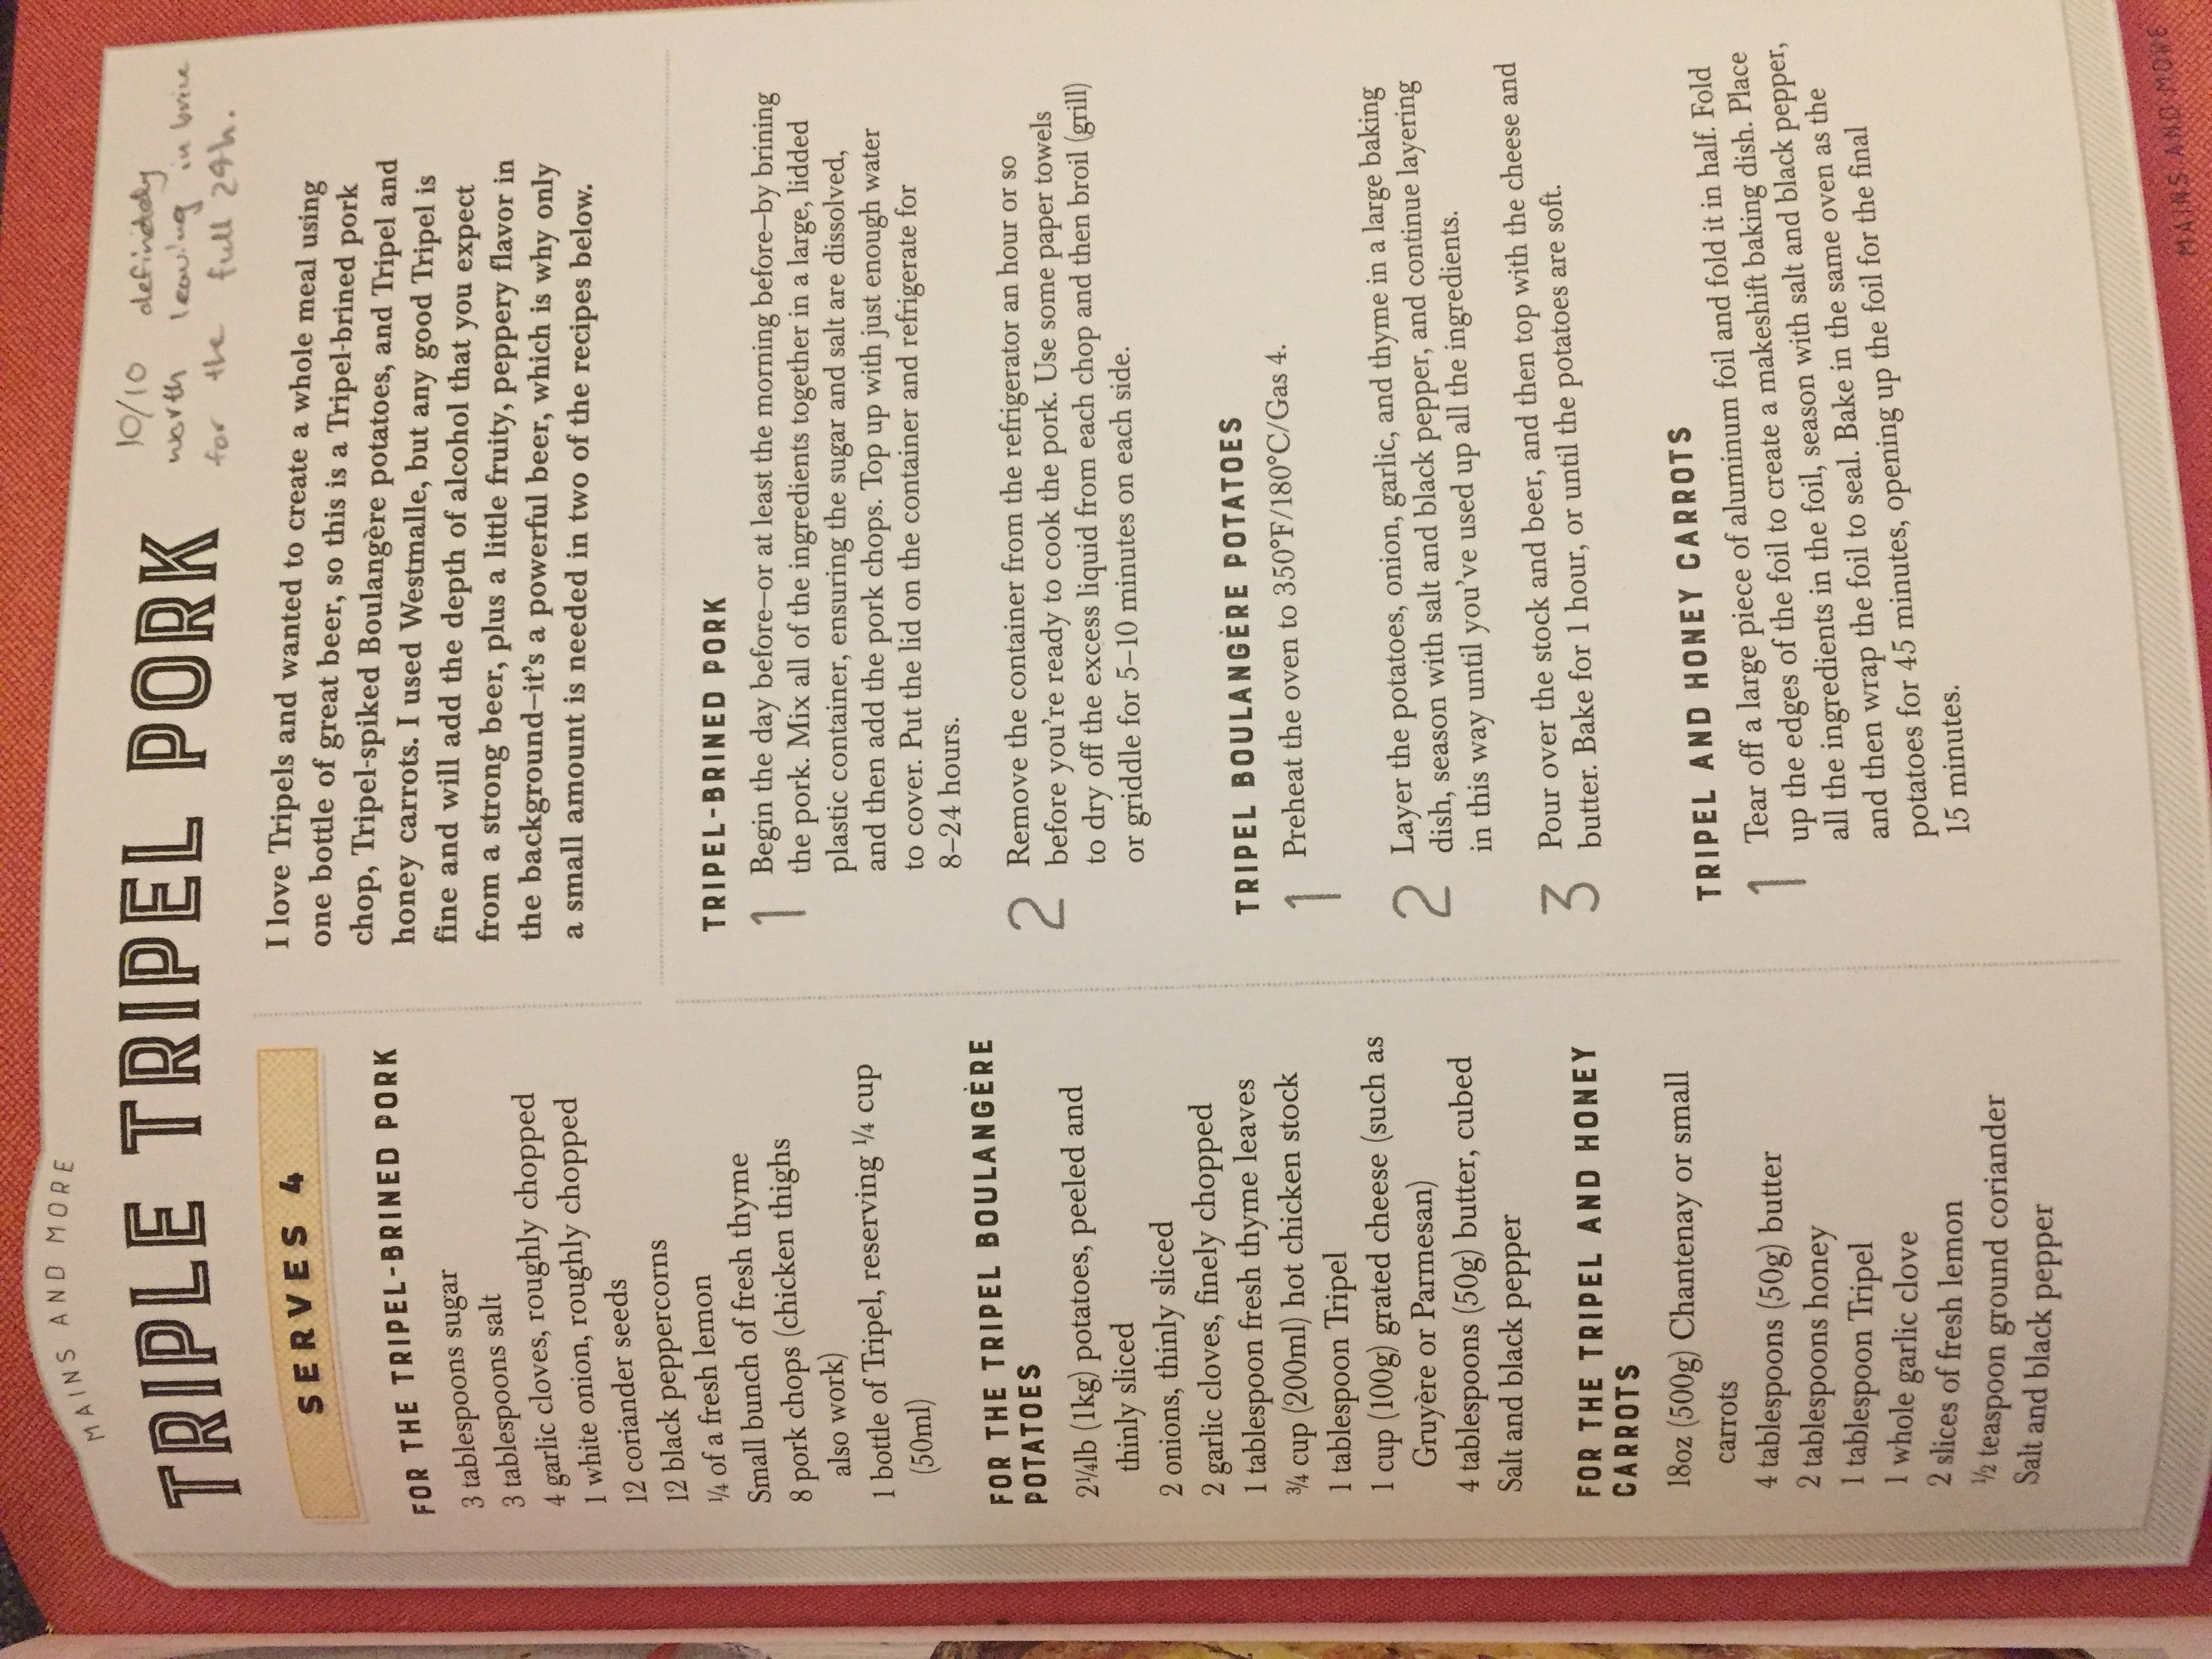
\includegraphics[height = 14cm, angle=270]{TripelPark}
  \end{center}
\end{figure}

\chapter{Turkey}
\section{15 minute Turkey Lasagne}
\begin{figure}[h!]
  \begin{center}
  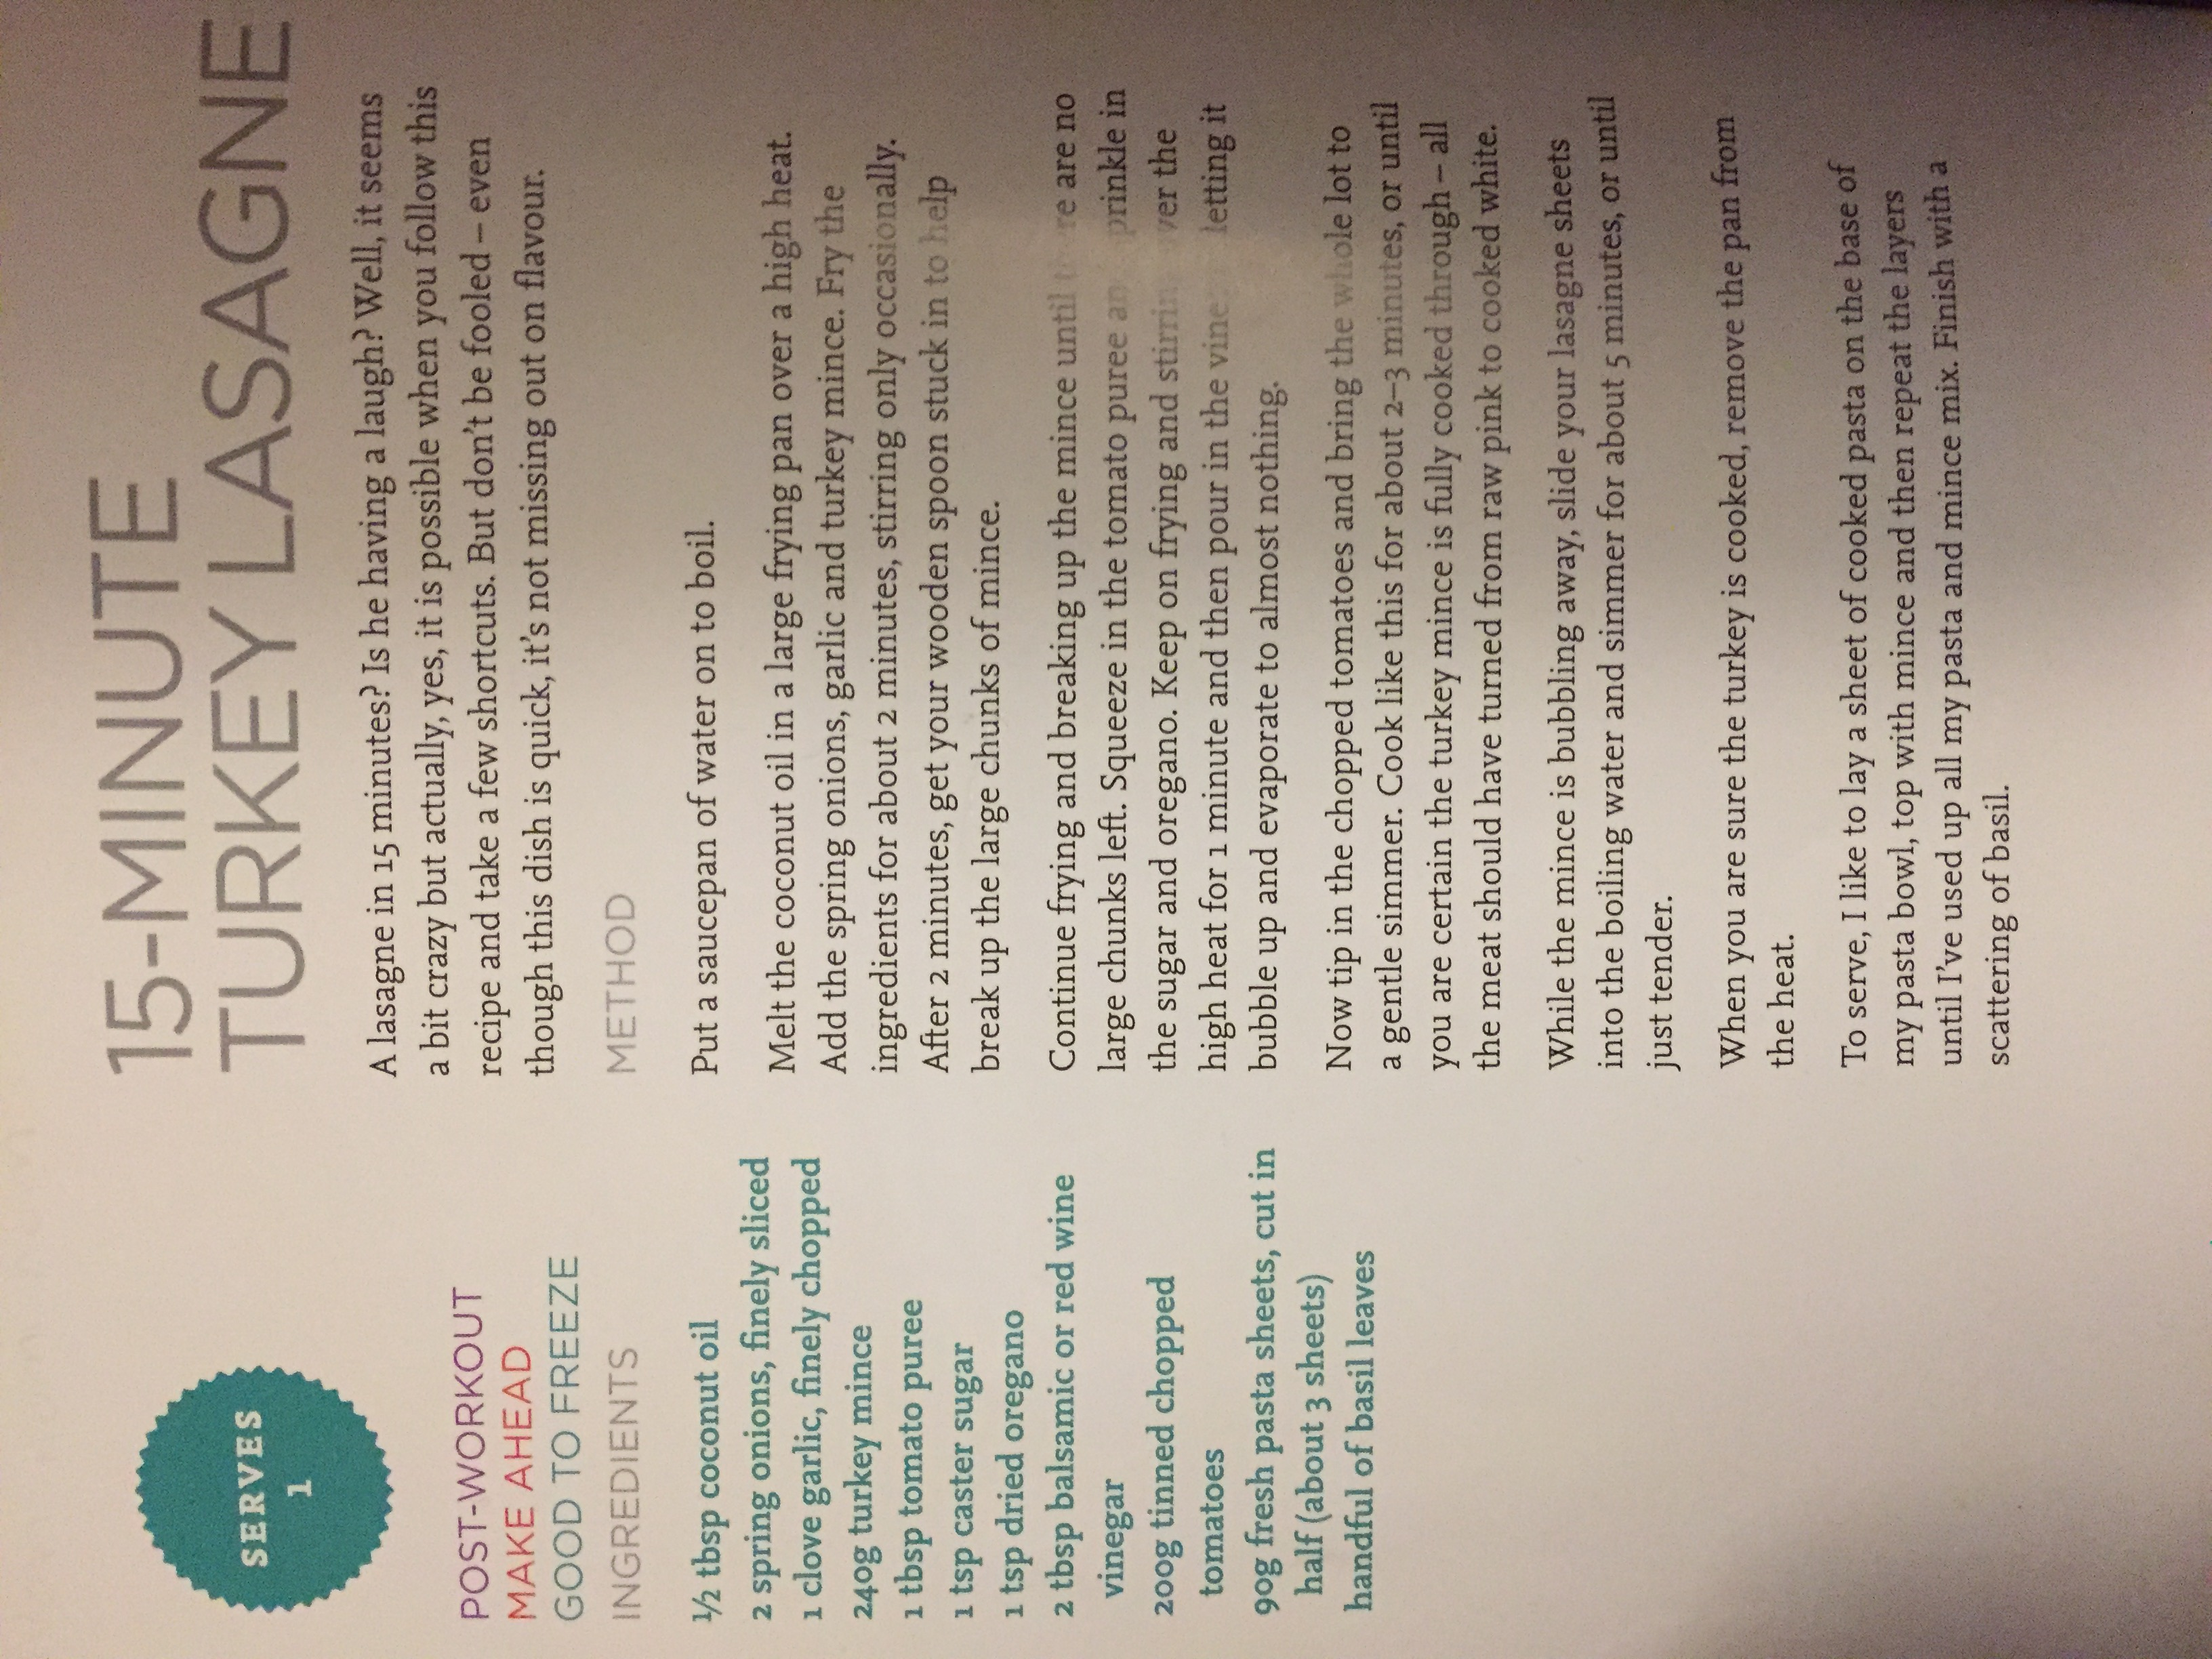
\includegraphics[height = 14cm, angle=270]{TurkeyLasagne}
  \end{center}
\end{figure}

\chapter{Vegetarian}

\section{Baked Gnocchi with Mushroom and Spinach}
\bf{Serves: 4} \\
\bf{Cooking Time: 1 hour} \\

\bf{Ingredients} \normalfont \\
1 pack of gnocchi \\
pinch of grated nutmeg \\
1/2 teaspoon of olive oil \\
200g mushrooms, slices \\
1 clove of garlic, crushed \\
200g young leaf spinach \\
2tbsp creme-fraiche \\
75g white mature cheese \\

Add gnocchi to pan of boiling water and cook for 2 minutes. Heat the oven to 180$^{\circ}$. Cook the sliced mushrooms in a pan with a little oil for 5 minutes, then add garlic and cook for another two minutes. \\

Mix the gnocchi, spinach and mushrooms with half the grated cheese and the creme fraiche and then place in an ovenproof dish. Top with the rest of the grated cheese and bake on the top shelf for 15--20 minutes. 

\section{Butternutsquash, Spinach and Stilton Quiche}
\bf{Serves: 4} \\
\bf{Cooking Time: ??} \\

\bf{Ingredients} \normalfont \\
500g butternut squash (this is the prepared weight, buy a 1kg squash) \\
Olive oil \\
3 cloves of garlic \\
200g spinach, washed \\
125ml single cream \\
100g greek yoghurt \\
2 medium eggs \\
125g stilton, cubed \\
You will also need shortcrust pastry, either homemade or shop bought \\

Cut squash into large chunks (about 3 cm) and place on a baking sheet. Drizzle with 2 tablespoons of olive oil and roast for 40 min (200$^{\circ}$C), until tender and caramelized at the edges. Remove and drain. (I never drain) \\

Heat 2 tablespoons of oil in a pan and gently fry the garlic, then add the spinach and toss well. It will cook in about 3 minutes. Remove from heat and season. \\

Place the cream, yoghurt, eggs and blue cheese in a food processor and blend briefly until well combined. Season with pepper, careful on the salt as the cheese contains a fair amount of salt. Arrange the squash and spinach over the pastry base and slowly pour over the blue cheese mixture. \\

Bake in the oven (190$^\circ$C ) for about 30 minutes or until golden brown. Serve barely warm with salad.

\section{Cannelloni with Spinach and Ricotta}
\bf{Serves: ??} \\
\bf{Cooking Time: ??} \\

\bf{Ingredients} \normalfont \\ 
Spinach, frozen is fine, you need to blanch and squeeze if you use fresh \\
500 gr if using frozen, 1kg if fresh \\
250 gr Ricotta \\
fresh thyme \\
Garlic \\
Freshly milled pepper \\
Shallot or finely diced onion \\
Cannelloni tubes \\
White sauce \\
Mozzarella \\

Mix onions, squeezed spinach and ricotta thoroughly and combine with the seasonings. Fill the dry cannelloni with the mixture and put into an ovenproof dish. Make the white sauce in the usual fashion and season with grated nutmeg. Pour sauce over the cannelloni and transfer dish to oven. Cook for 20 min or until the cannelloni are cooked. 10 min before end of cooking sprinkle Mozzarella or any other cheese available over the dish.

Buon appetito


\section{Jaime Oliver's Quorn \& Leak Stew}
\label{vegversion}


\textbf{Serves: 4} \\
\textbf{Cooking Time: ?} \\ 

\textbf{Ingredients}\\ 
2 tblsp extra-virgin olive oil \\
2 medium leeks, white and tender green parts only, thinly sliced \\
200-300g cremini mushrooms, thinly sliced \\
Salt and freshly ground pepper \\
1 pack of Quorn `chicken' pieces \\
1 1/2 cups vegetable stock \\
1 tblsp chopped thyme \\ 
2 tblsp sour cream \\
2 tsp Dijon mustard \\

\textit{Serve with garlic bread and rice/potatoes} \\

In a pan, heat 1 tablespoon of the oil. Add the leeks and cook over moderate heat, stirring, until softened, about 7 minutes. Add the mushrooms and season with salt and pepper. Cover and cook, stirring, until the mushrooms are tender, about 4 minutes. Scrape the leeks and mushrooms onto a plate. \\

Season the quorn with salt and pepper and lightly dust with flour, shaking off any excess. Heat the remaining 1 tablespoon of oil in the skillet. Add the quorn and cook over moderate heat until golden brown, about 2 minutes per side. Add the stock and thyme and simmer over moderate heat until the quorn is just cooked through, about 1 minute. Using a slotted spoon, transfer the quorn to the plate with the vegetables. \\

Simmer the stock over moderately high heat until reduced by half, about 2 minutes. Return the quorn, leeks and mushrooms to the skillet and simmer over low heat until warmed through, about 1 minute.  \\

In a small bowl, blend the sour cream with the mustard (Alistiar says 2tsp is too much apparently but I liked it) and stir into the stew. Remove the skillet from the heat. Season the stew with salt and pepper and serve. Serve With new potatoes or steamed rice and garlic bread.

\section{Layered Pasta Bake}
\bf{Serves: ??} \\
\bf{Cooking Time: 40} \\

\bf{Ingredients} \normalfont \\ 
400g tinned, chopped tomatoes \\
115g tomato puree \\
200ml water \\
2 teaspoons dried thyme or 1 teaspoon fresh chopped \\
2 cloves garlic \\
10 sundried tomatoes, chopped \\
200g Feta, diced \\
350g Pasta (Fusili or Penne) \\
1 medium Onion \\
3 medium courgettes, sliced \\
3 Tablespoons Olive Oil \\
50g Cheddar \\
chopped fresh basil \\

In a saucepan make the tomato sauce by simmering the chopped tinned tomatoes, tomato puree and water with the thyme, garlic and the sundried tomatoes. When the sauce has reduced and thickened (around 8--10 min) add the Feta and season to taste.\\

Cook the pasta al dente, drain and mix thoroughly with the tomato sauce. In a saucepan sauté the onions and courgettes in olive oil for 2-3 min. Spread half of the pasta mix into a casserole dish and layer the courgette mix on top. Cover with the remaining pasta and sprinkle the cheddar and bake at 180$^{\circ}$C in the oven for 20--25 min. \\

Serve hot. Sprinkle with the fresh Basil if you can be bothered.
  

\section{Macaronni Cheese}
\textbf{Serves: 4} \\
\textbf{Cooking Time: 40} \\

\textit{non-veggie version: add in bacon or smoked sausage. \\
spicy version: add in some jalapenos. \\}

\textbf{Ingredients} \\
2 tbsp butter \\
piece of bread \\
350g spiral or other short pasta \\
1 garlic clove, finely chopped \\
1 tsp English mustard powder \\
3 tbsp plain flour \\
500ml whole milk \\
250g mature cheddar, grated \\
50g Parmesan \\
handful of brocolli \\
half sausage (Matheson smoked) \\

Heat oven to 200$^\circ$C. Spread the chunks of bread over a baking sheet, drizzle with the melted butter and season. Bake for 6 mins until crisp, then set aside. \\

Boil the pasta for 2 mins less than stated on the pack. Meanwhile, melt the remaining butter in a saucepan. Get the brocolli boiling in a pan until cooked. Add the garlic and mustard, cook for 1 min, then stir in the flour. Cook for 1 min more, then gradually whisk in the milk until you have a lump-free sauce. Add the sausage, and brocolli, simmer for 5 mins, whisking constantly until thickened. Take off the heat, then stir in all the cheddar and half the Parmesan.\\

Stir the pasta and some seasoning into the cheesy sauce, then tip into a large ovenproof dish. Scatter over the bread and remaining Parmesan, then bake for 20 mins until crisp and golden. Can be frozen before baking – defrost thoroughly before cooking. \\
   
\section{Marillen Knoedel}
\bf{Serves: ??} \\
\bf{Cooking Time: ??} \\

\bf{Ingredients} \normalfont \\
\it{F\"{u}r der Teig}: \normalfont \\
60g weiche Butter \\
250g Quark           \\                 
125g Weizenmehl   \\
10 kleine Aprikosen \\
Wuerfelzucker \\

\it{F\"{u}r der Sosse}: \normalfont \\
70g Butter \\
70g Semmelbroesel \\
30g Zucker \\
1 Paeckchen Vanillezucker \\

Butter und Quark geschmeidig ruehren. Dann das Mehl unterruehren und eine Stunde im Kuehlschrank kuehlen. Aus dem Teig eine Rolle formen und in 10 Stuecke schneiden. Die Fruechte entkernen und ein Stueckchen Zucker in die Mitte geben und mit dem Teig zu Knoedeln formen. In kochendes Salzwasser geben und etwa 15 min garen lassen. \\


Lass die sosse unter ruehren leich roesten und die Knoedel darin waelzen. Mit zerlassene Butter und Aprikosenkompott servieren. An guaden, wie sie in Bayern sagen wuerden. \\

\section{Pumpkin baked with couscous and goat cheese}
\bf{Serves: 4} \\
\bf{Cooking Time: 1.25 hr} \\


\bf{Ingredients} \normalfont \\
2kg pumpkin \\
2tbsp olive oil \\
125g bulgur wheat or couscous, rinsed \\
300ml hot vegetable stock \\
1 onion, chopped \\
3 gloves of garlic, finely chopped \\
small bunch flat-leaf parsley, roughly chopped \\
small handful of chives, roughly chopped \\
100g of hard goat's cheese \\

Preheat the oven to 200$^{\circ}$C. Slice off the top quarter of the pumpkin (you can use this flesh for something else - pumpkin pancakes?) and scoop out the seeds (baked pumpkin seeds?). Put the pumpkin on a baking tray and brush the inside with olive oil. Bake in the oven for 30 minutes. \\

Meanwhile, put the couscous in a heatproof bowl and cover with the vegetable stock. Cover and set aside for 20 minutes, drain if necessary. \\

Heat the remaining 1tbsp olive oil in a small frying pan over a medium-high heat. Add the onion and fry for one minute before adding the garlic. Cook for 2-3 minutes until softened. \\

Stir the onion mixture parsley and most of the goats cheese into the couscous and season well. Remove the pumpkin from the oven and reduce the temperature to 180$^{\circ}$. Spoon the mixture into the pumpkin and top with the remaining cheese. Return to the oven for a further 30 minutes or until golden. Serve scattered with the remaining chives. \\

\begin{figure}[h!]
  \begin{center}
  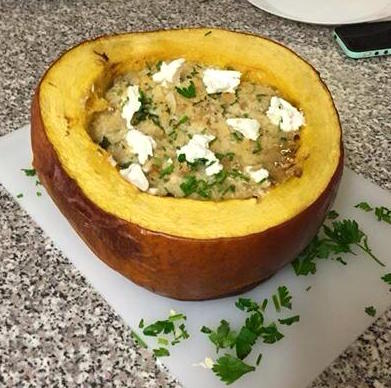
\includegraphics[height = 10cm]{bakedpumpkin}
  \end{center}
\end{figure}

\section{Sour Chickpeas}
\bf{Serves: 6} \\
\bf{Cooking Time: ??} \\

\bf{Ingredients} \normalfont \\
350g chickpeas \\
1.75 l water \\
2.5 tspn salt \\
275-300g onions, peeled and finely chopped \\
1 hot green pepper, finely chopped \\
1 tblsp ginger finely grated \\
4 tblsp lemon juice \\
6 tblsp vegetable oil \\
225g tomatoes finely chopped \\
1 tblsp ground corriander \\
1 tblsp ground cumin \\
1/2 tspn ground turmeric \\
2 tspn garam masala \\
1/4 tspn cayenne pepper \\

Remove chickpeas from their liquid. Put 2 tablespoons of the chopped onions, 1/2 teaspoons of the salt and the green chilli, ginger and lemon juice into a teacup. Mix well and set aside. \\

Put the oil in a heavy, wide, casserole type pan and set over medium-high heat. When hot, put in the chopped onions. Stir and fry for 8-10 minutes or until onion bits turn red/brown. Add the tomatoes. Continue to stir and fry for another 5-6 minutes, mashing the tomato pieces with the back of a slotted spoon. Put in the coriander, cumin, turmeric. Stir and cook for about 30 minutes. Now put in the drained chickpeas, 400ml of their cooking liquid, the remaining 2 tspn of salt, the garam masala and cayenne. Stir to mix and bring to a simmer. Cover, turn heat to low and cook very gently for 20 mins. Stir a few times during this period. Add the mixture in the teacup. Stir again to mix.Serve hot or lukewarm. 




\section{Spicy festive strudel with Apricots and Stilton}
\bf{Serves: ??} \\
\bf{Cooking Time: ??} \\

\bf{Ingredients} \normalfont \\
1 parsnip, peeled, woody core removed \\
1 carrot, peeled \\
1 small leek, trimmed, washed and cut into thin strips \\
\nicefrac{1}{2} small swede, peeled \\
2 small turnips, peeled \\
1 small sweet potato, peeled \\
115g butter \\
1 onion, peeled and chopped \\
pinch of ground cumin \\
pinch of ground cinnamon \\
pinch of ground allspice \\
zest of 1 lemon \\
10 ready to eat apricots, chopped \\
115g Stilton, crumbled \\
2 tablespoons of chopped fresh coriander \\
salt, pepper \\
270g frozen filo pastry sheets, thawed \\

Cut all the root vegetables into matchstick size pieces. Bring a large saucepan of salted water to the boil, add veggies and cook for 3 min. Keep them al dente as they still get a blast in the oven. Drain. \\

Melt a little butter in a large frying pan and sauté  the onion until translucent. Add the spices,  lemon zest and veggie sticks, then stir fry for 2 min. (I prefer to do that in batches so veg stays crisp) Allow the mixture to cool then stir in the stilton and coriander. Season well with salt and black pepper. \\

Preheat oven to 200 degree. Melt the remaining butter. Unfold one sheet of filo pastry and lightly brush with butter. Place a second sheet on top, brush again and continue until all filo pastry is utilized. \\

Spread veggie mix down the centre, gently fold in ends and long sides so you have a log. Turn the parcel so the seme-side is down and brush with a little more butter. Sprinkle with some salt if you wish. Bake in the oven for 30--40 min until crisp and golden. Serve at once. \\

\begin{quote}
  \it\centering{Some hae meat and cannae eat, \\
Some can eat but want it, \\
But we hae nae meat, \\
And we can eat, \\
So may the lord be thanket,} \normalfont
\end{quote}
 
\section{Spinakopitakia}
\bf{Serves: 4} \\
\bf{Cooking Time: 50 mins} \\

\bf{Ingredients} \normalfont \\
1 Paket Blaetterteig \\
500gr Spinat (tiefgefroren ist ok) \\
2 Lauchzwiebeln \\
300 gr griechischer Schafskaese (Feta) \\
4 Eier \\
1/8 ltr Milch \\
1 Bund Petersilie \\
50 gr zerlassene Butter \\
Sesam \\

Spinat auftauen, gut ausdruecken und klein hacken. Mit frischem Spinat in einem grossen Topf ca 3 Minuten zugedeckt garen und dann auf einem Sieb abtropfen lassen. Die Lauchzwiebeln/ Fruehlingszwiebeln putzen, waschen und in duenne Ringe schneiden. \\

Oel erhitzen, Zwiebeln und Spinat darin bei mittlerer Hitze etwa 2 Minuten schmoren. Mit Salz, Pfeffer und Muskat wuerzen und lauwarm abkuehlen lassen. Fein zerkruemelten Schafskaese, Eier und gehackte Petersilie untermischen. \\

Feuerfeste Form mit zerlassener Butter auspinseln und etwa 2/3 des Blaetterteiges in Schichten auslegen. Dabei jeweils die einzelne Lage mit zerlassener Butter bestreichen.  Spinatfuellung darauf glatt streichen. Nun die restlichen  Blaetterteigplatten auslegen. \\

Kuchen in Portionsstuecke schneiden, mit Milch betraeufeln und mit Sesam bestreuen. Bei 200 Grad etwa 40 Minuten backen bis er schoen braun ist. \\

Lauwarm oder kalt servieren. Dazu passt Tomaten oder Gurkensalat. \\

Ganz einfach!


\chapter{Venison}

\section{Salt Plum Venison Seasoned Haunch of Venison with Ginger-Poached Pears}
\bf{Serves: 4--6} \\
\bf{Cooking Time: ??} \\

\bf{Ingredients} \normalfont \\
Small, boned hauncg of venison ($\approx$ 900g for 4--6 people)\\
5--6 plums or 1 rounded tbsp of umeboshi puree \\
1 tbsp soy sauce \\
1 tbsp honey \\
2 tbsp olive oil \\

\textbf{For the poached pears} \\
250g golden caster sugar \\
200ml water \\
5cm piece of ginger root, peeled \\
4 firm pears \\


Cut into the meat, but not all the way through, just to graze it. Blend the plums into a puree and spred this over all of the meats surface. then roll up the meat and tie with string or secure with cocktail sticks. Whisk together the soy sauce, honey and olive oil and pour over the meat. Leave this to marinade at room temperature for a couple of hours or overnight in the fridge. \\

Preheat the oven to 230$^{\circ}$C and place the joint and marinade in a roasting dish and roast for 25 minutes (or around 25 minutes per kilo). Then rest the meat in a warming oven or over a warm hob and lightly tented with foil, for 25 minutes. \\

Baste it with the pan juices. In a large saucepan, dissolve the sugar in the water and bring to the boil and add peeled and thickly sliced ginger. Simmer for a few minutes. Peel, half and core the pears and slip them into the syrup. Cook gently until tender and translucent, 10--25 minutes. Remove and slice thickly to serve. Untie the meat and slice. Serve with a pear half and with baked or roast potatoes with beans. 

\section{Venison Brioch}
\bf{Serves: 4} \\
\bf{Cooking Time: ??} \\

\bf{Ingredients} \normalfont \\
1.5 pounds of diced haunch of venison \\
1/2 pint of red wine \\
1 finely chopped onion \\
6 bayleafs \\
1 chopped carrot \\
12 peppercorns \\
1 stick of celery \\
2 oz. butter \\
1 tbsp tomato puree \\
2 oz. flour \\
1/2 pint of beef stock \\
2 apples \\
4 slices of bread \\
1 tbsp redcurrant jelly \\
1 tbsp plum jam \\
1 gill whisky \\

Place diced venison in red wine with carrot onion celery, bayleaf, peppercorns, leave for 2 days in the fridge, stir twice a day. Drain the venison from the marinade, seal in butter until golden brown, add tomato puree and flour, slowly add marinade and beef stock, cook slowly for 45 minutes. \\

Peel apples, cut in half and poach. Cut bread into four circles and fry until golden brown. Place a little redcurrant jelly on each crouton. Add plum jam to venison and season. Place croutons on serving dish, pour venison on top, place half an appl on each portion and flame with the whisky. 

\part{Deserts}

\section{Any flavour Ice Cream}
\bf{Serves: ??} \\
\bf{Preparation Time: ??} \\ 

\bf{Ingredients} \normalfont \\
1 pint heavy whipping cream \\
400ml (14Oz) sweetened condensed cream \\
any flavouring - honey, chocolate, berries, caramel \\

Whisk the whipping cream until it forms soft peaks. The add the condensed milk then whisk well. The add whatever flavouring you want. Then freeze for 6 hours. 


\section{Bailey's Cheesecake}
\bf{Serves: 10--12} \\
\bf{Preparation Time: 10 minutes, Cooking Time: 2 hours} \\ 

\bf{Ingredients} \normalfont \\ 
100g butter \\
250g digestive biscuits, crushed \\
600g cream cheese \\
25ml Baileys or other Irish cream liqueur \\
100ml icing sugar \\
300ml double cream, whipped \\
100g grated chocolate \\
200ml double cream, whipped \\
cocoa powder, to dust \\ 

Melt the butter in a pan and add the crushed digestive biscuits. Mix well until the biscuits have absorbed all the butter. Remove from the heat and press into the bottom of a lined 18cm spring-form tin. Place in the refrigerator and allow to set for one hour. \\

Meanwhile, prepare the filling. Lightly whip the cream cheese then beat in the Irish cream and icing sugar. Fold in the whipped cream and grated chocolate. When smooth, spoon evenly onto the biscuits.Refrigerate and allow to set for a further two hours. Once set, remove and decorate with whipped cream and cocoa powder dusted over the top. Serve.

\section{Chocolate Orange Cake}
\bf{Serves: 6--8} \\
\bf{Cooking Time: ??} \\ 

\bf{Ingredients} \normalfont \\ 
115g Self Raising flour \\
25g cocoa \\
1 tsp baking powder \\
115g soft margarine \\
85g caster sugar \\
25g golden syrup \\
Grated Zest of 1 orange, plus 2 tblsp of the juice \\
2 eggs, beaten \\
55g plain chocolate chips \\

\it{To Decorate} \normalfont \\
25g chopped walnuts \\

Preheat the oven to 180$^{\circ}$C \\

Place all the cake ingredients into a basin and beat thoroughly. Turn into a greased 18cm round tin. Then Sprinkle over the chopped walnuts. \\

Bake in the centre of the oven for around 40--45minutes until risen and well cooked. 
Rest in the tin for 10 minutes and then remove from the tin and allow to cook on a 
wire rack. \\

\bf{Variations} \normalfont \\
Substitute the walnut decoration for buttercream topping and decorate with curls 
of chocolate. 


\section{Cranachan with Raspberries}
\bf{Serves: ??} \\
\bf{Cooking Time: ??} \\

\bf{Ingredients} \normalfont \\ 
125g of oats \\
75g light muscovado sugar\\
3--4 tbsp malt whisky and extra to serve \\
250g mascarpone \\
300ml double cream, lightly whipped \\
250g raspberries \\
honey, optional \\

Put the oats and sugar on a large sheet of foil and place under a hot grill for three to four minutes stirring every 30 seconds or so. They do burn easily so watch carefully then remove and cool. Add whisky to the mascarpone according to taste and beat well until smooth. Fold this into the cream with the cooled oat mixture. Once thoroughly combined, gently fold in the raspberries, taking care not to break them up. Tip into a glass bowl, cover and serve at once - or chill for no more than an hour. Serve in bowls with an optional drizzle of whisky - and a spoonful of honey. 

\section{Easy Chocolate Mousse}
\bf{Serves: ??} \\
\bf{Cooking Time: 40} \\

\bf{Ingredients} \normalfont \\ 
2 Tafeln Schokolade (1 Vollmilch und 1 Dunkel) 
(Translation: tafeln = bar) \\
200-250ml Sahne (whipped or double cream in UK) \\

Sahne schlagen. 
Die Schokolade in der Bain Marie schmelzen. (Nicht mit der Schokolade ins Bad sondern die Schokolade in einer feuerfesten Form in einem Topf mit heissem Wasser  langsam und unter Ruehren schmelzen). \\

Die noch heisse geschmolzene Schokolade vorsichtig unter die Sahne heben. Entweder in einer Form, oder in individuellen zum beispiel Mokkataesschen abkuehlen lassen. \\

\section{Ginger Coffee Cake}

\begin{figure}[h!]
  \begin{center}
  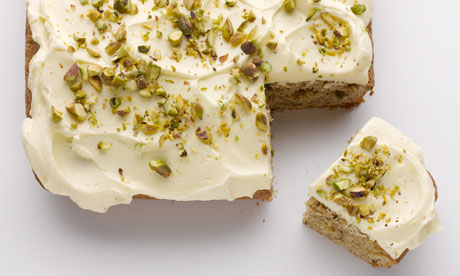
\includegraphics{coffeecake}
  \end{center}
\end{figure}

\bf{Serves: ??} \\
\bf{Cooking Time: 40} \\

\bf{Ingredients} \normalfont \\
175g unsalted butter \\
75ml milk \\
1 tbsp ground coffee (not instant) \\
2cm piece root ginger, finely grated \\
2 large eggs \\
225g caster sugar \\
100ml sunflower oil \\
100g chopped pistachios \\
275g plain flour \\
3 tsp baking powder \\
200g cream cheese \\
Finely grated zest of 1 lemon \\
2 tsp lemon juice \\
175g icing sugar \\
 
Our baking guru says coffee and fresh ginger are a marriage made in heaven. And who are we to disagree? \\

Line the base and sides of a deep, 22cm square baking tray or cake tin with nonstick paper, and heat the oven to 180C (160C fan-assisted). In a pan, melt 50g butter, remove from the heat, stir in the milk, coffee and ginger, and set aside. Whisk the eggs and sugar until foamy and pale, then beat in the coffee mix and oil. Stir in 75g pistachios, fold in the flour and baking powder, and spoon into the tin. Bake for 30-35 minutes, until a skewer comes out clean, and leave to cool. \\

Beat the remaining butter until smooth and light, then beat in the cheese, zest and juice, followed by the icing sugar. Spread over the top of the cold cake and decorate with the remaining nuts. \\

The sharp kick of fresh ginger root is stupendous with coffee. Add finely chopped glacé ginger or dried apricots to make it fruitier, if you like.  \\

\section{Grandmas chocolate truffles}
\bf{Serves: ??} \\
\bf{Cooking Time: ??} \\

\bf{Ingredients} \normalfont \\ 
225g good plain chocolate \\
25g caster sugar \\
50g butter \\
2 tblsp rum \\ 
1 large egg yolk \\
cocoa powder \\
decimated coconut \\
vermicelli (chocolate sprinkles/shreds) \\

Break chocolate into a bowl, melt in double saucepan. Then stir in sugar, butter, rum and egg yolk and beat until mixture is thick and cool. Shape into small balls and divide into 3 lots. Roll into: \\

1. cocoa \\
2. vermicelli \\
3. coconut \\

\begin{figure}[h!]
  \begin{center}
  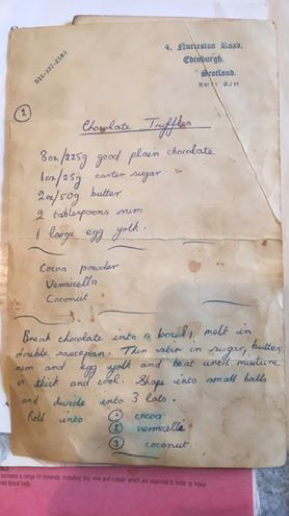
\includegraphics[width = 10cm]{Picture1.png}
  \end{center}
\end{figure}


\section{Honeycomb chocolate brownie}
\bf{Serves: ??} \\
\bf{Cooking Time: ??} \\

\bf{Ingredients} \normalfont \\ 
450g caster sugar \\
50 ml runny honey \\
1 tblsp liquid glucose \\
50ml water \\
3/4 tspn bicarbonate of soda \\
150g butter \\
200g dark chocolate \\
3 eggs \\
115g plain flour \\

Put the 200g sugar, honey, liquid glucose, water in a pan. Simmer until you have golden caramel. Then add the bicarbonate of soda then mix well. Pour this mixture into a grease-lined brownie tin. Leave this to set for 30 mins. \\

Melt the butter and dark chocolate. Mix the rest of the sugar (250g) and 3 eggs and add the butter/chocolate mix. Mix well then add the flour and again mix well. Smash up the set honey mixture into small pieces. Stir these into the chocolate  and mix. Then pour this into a greased brownie tin. \\

Bake for 25 mins at 180 degrees then leave to cool for a little. 

\section{Lemon Drizzle Poppy Seed Cake}
\bf{Serves: 12 slices} \\
\bf{Cooking Time: 1 hour} \\

\bf{Ingredients} \normalfont \\ 
175g butter, softened, plus extra for greasing \\
175g golden caster sugar \\
200g self-raising flour \\
4 lemons, zested and 2 juiced for icing \\
3 eggs \\
2 tbsp poppy seeds \\
125g pot natural yoghurt \\
\it{For the icing } \normalfont \\
200g icing sugar \\
3 tbsp lemon juice \\

Heat oven to 180C/160C fan/gas 4. Grease and line the base of a 20cm square deep cake tin (or if using a decorative tin like ours, grease well). \\

In a bowl, beat the butter and sugar until fluffy. Add the rest of the ingredients and beat until combined. Spoon into the tin and smooth over the top. Bake for 40-45 mins. Cool in the tin for 10 mins, then turn out, peel off the parchment and leave to cool on a wire rack. \\

Sift the icing sugar into a bowl. Beat in the lemon juice to make a runny icing. Pour over the cake and leave to set. \\

\section{Luciakatern}
\textbf{Makes: 30--35} \\
\textbf{Cooking Time: ??} \\

\textbf{Ingredients}  \\
60g yeast\\
1/2 l milk \\
200g butter \\
2 eggs\\
1 tsp salt \\
200g sugar \\
1/2 tsp saffron \\
50g chopped almonds \\
1kg flour \\
raisons \\

Break up the yeast in a bowl and mix with some of the milk. Whisk one egg and add to the bowl. Melt the butter and heat with the rest of the milk until lukewarm. Pour this over the yeast and then add the salt, sugar and saffron. Add the flour and almonds to this a bit at a time, all the while mixing the dough. Leave this until it doubles in size (15--20 minutes). \\

Knead the dough again and shape it into your 30 cats/men.  Leave these again to allow them to rise a little. Whisk the second egg and use this to glue the raisons onto the cats/men as eyes. Use the rest of the egg as a wash to coat the dough. Bake in the oven for 10 minutes at 200$^{\circ}$. 

\section{Malteser Chocolate Cake}
\textbf{Serves: 8--10} \\
\textbf{Cooking Time:25-30 minutes} \\

\textbf{Ingredients} \\ 
\textit{for the sponge} \\
50g really soft butter \\
250g caster sugar \\
150g self-raising flour \\
125ml sour cream \\
4 medium eggs \\
50g cocoa powder \\
1 tsp baking powder \\
pinch of salt \\
half a vanilla pod (or few drops of vanilla extract to taste) \\

\textit{for the buttercream} \\
100g dark chocolate \\
550g icing sugar \\
250g really soft butter \\
2 tbsp milk \\

\textit{for the decorate} \\
4 x 135g packets of Maltesers \\

Preheat the oven to 160C. Grease 2 x 20cm sandwich cake tins with a little butter. Put the butter, sugar, flour, sour cream, eggs, cocoa powder, baking powder and salt in a large bowl. Split the vanilla pod open, scrape out the seeds and add them too (or the vanilla extract). Then mix or blend to give a smooth, soft mixture. Divide evenly between the cake tins, smooth the tops and place in the oven for 25-30 minutes.\\

Check if the cakes are baked by inserting a skewer into the middle. Remove them from the oven and leave to cool on a wire rack for about 25 minutes. When the cakes are almost cool, start making the buttercream. Break the chocolate into a medium bowl and melt it in the microwave in 30-second blasts, stirring inbetween. Otherwise, sit the bowl of chocolate on a medium pan of simmering water, making sure that the water does not touch the bottom of the bowl, as this may make the chocolate grainy. \\

Sift the icing sugar into the electric mixer bowl. Add the butter and milk (or water) and beat until it is really light and fluffy.  Then pour in the melted chocolate, stirring all the time. 

Sit one of the cakes on a serving plate then put about a third of the buttercream on and spread it around. Then sit the other sponge on top and spread the remaining buttercream all over so it is completely covered. Then take the Maltesers and stick them all over the cake. \\

\section{Markthalle Germkn\"{o}del}
\textbf{Serves: ??} \\
\textbf{Preparation Time: 1.5 hours, Cooking Time: 20 minutes} \\

\textit{F\"{u}r die Kn\"{o}del} \\
1 packet instant yeast (2 1/4 tsp.), dried yeast works, in which case proof with milk before adding to the flour \\
500g all-purpose flour \\
1/2 c. sugar \\
1 tsp lemon zest \\
2 T. vanilla sugar or sugar plus 1/2 tsp. vanilla extract \\
1/2 tsp. salt \\
1 egg \\
5 T. butter, softened \\
1 c. lukewarm milk \\

\textit{For the Filling} \\
3/4 c. plum jam \\
1 T. rum (optional) \\
1/4 tsp. cinnamon (optional) \\

\textit{For the topping} \\
1/3 c. poppy seeds \\
1/3 c. sugar \\

\textit{Start the dough}: Mix the instant yeast with the flour, sugar, vanilla sugar, lemon zest and salt. Add the softened butter, egg and milk and mix, using a dough hook or with a spoon by hand, until a medium-soft dough forms. Adjust flour or milk as needed to make a pliable, but not sticky dough. If you are making the dough by hand, turn it out on a lightly floured board and knead for several minutes, until smooth and elastic. If dough is too stiff, knead with wet hands until it becomes softer. Form the dough into a ball, flour lightly and place in a bowl to double in a warm place. Cover with a clean towel. Let it rise about 1 hour, or until doubled in size. The dough made with instant yeast might rise faster. \\

\textit{Make filling}: If you are adding rum and / or cinnamon to the jam, stir it together now. You may use any jam flavour or cherries or Nutella, too. \\

\textit{Form dumplings}: Remove your dough from the bowl to a lightly floured board. Pinch off 50-60 grams. You may make them larger, but they will take longer to steam. Roll the pieces into a ball and then flatten them with your palm to form 10cm circles. Add 2 teaspoons of jam to the centre and then pull up opposite sides and pinch closed. Pinch the other two sides closed and make sure the jam is well-sealed inside the dough. Roll the dumplings bit in your hands to round up the dumpling. Set dumplings on the floured board, sprinkle with flour if you wish, and cover with a cloth. Let sit 10--20 minutes. \\

Prepare your steamer: Place 1 to 2 inches in the pan, hang the steamer over the water and bring the whole thing to a boil (you will need a lid, too). Steam --- Place dumplings on steamer over boiling water, leaving about 1 inch of room to rise in all directions. Cover pan and steam 20 minutes. You may also make vanilla sauce while you are waiting for the dough to rise.\\

Make topping: You can leave your poppy seads whole, otherwise, grind equal amounts of poppy seeds and sugar in a poppy seed grinder or a blade coffee grinder. Set aside. \\

Serve: Place 1 or 2 dumplings on a plate and pour melted butter over the top. Sprinkle poppy mixture over top, as much as you wish. Pour vanilla sauce and poppy mixture over the top when you are ready.

\section{Marbled Pumpkin Cheesecake}

\it{This tastes much better than it looks......I have been told it was the best cheesecake ever eaten by multiple sources.} \\

\bf{Makes: 12 large} \\
\bf{Cooking Time: 1 hour 40 minutes} \\

\bf{Ingredients} \normalfont \\ 
80g crushed ginger nut biscuits \\
60g finely chopped pecans \\
75g butter, melted \\
450g cream cheese, softened \\
150g caster sugar, divided \\
1 teaspoon vanilla extract \\
3 eggs \\
250g pumpkin puree \\
3/4 teaspoon ground cinnamon \\
1/4 teaspoon ground nutmeg \\

Preheat the oven to 180 C / Gas mark 4. In a medium bowl, mix together the crushed gingernut biscuits, pecans and butter. Press into the bottom, and about 2.5cm up the sides of a 23cm (9 in) springform tin. Bake base 10 minutes in the preheated oven. Set aside to cool. \\

In a medium bowl, mix together the cream cheese, 100g of the sugar and vanilla just until smooth. Mix in eggs one at a time, blending well after each. Set aside 250ml of the mixture. Blend remaining sugar, pumpkin, cinnamon and nutmeg into the remaining mixture.
Spread the pumpkin mixture into the base, and drop the plain mixture by spoonfuls onto the top. Swirl with a knife to create a marbled effect. \\

Bake 55 minutes in the preheated oven, or until filling is set (I find that this is actually shorter than 55 minutes so keep an eye on it!). Run a knife around the edge of the tin. Allow to cool before removing tin rim. Chill for at least 4 hours before serving.

\section{Meringues avec Hazelnut}
\bf{Makes: 12 large} \\
\bf{Cooking Time: 2 hours} \\

\bf{Ingredients} \normalfont \\ 
100g hazelnuts \\
4 egg whites \\
225g caster sugar \\


Note: To make plain meringues just leave out the hazelnuts. Preheat oven to 190$^{\circ}$. Roast the nuts for 5--10minutes until golden and leave to cool. Lower the oven to 110$^{\circ}$. Chop 8 nuts and set aside and put the rest into a food processor. Whizz with 1 tablespoon of sugar until roughly ground but don't overdo it as they will become oily. \\

For the meringues: Use a glass bowl. Separate the eggs ---- we want the egg whites obviously! Each egg white will lead to $\approx$ 3 large meringues. Whisk the egg whites into soft peaks --- it should stand in stiff, pointed peaks when you pull out the beaters. Do not over-beat or you will lose your air. Whisk in half the sugar, 1 tablespoon at a time, into the mixture until stiff. Then carefully add in the rest of the sugar as well as the blended hazelnuts with a large metal spoon. \\

Drop spoonfuls of the meringue mixture (spaced well apart) onto baking paper on a baking tray. Now sprinkle the 8 chopped hazelnuts on top. Then bake in the oven for 1.5--2 hours until they are dry and lift easily from the paper. Leave to cool at room temperature. Serve with whipped cream and raspberries. 

\section{Peanut Butter and Chocolate Lava Cake}
\bf{Serves: ??} \\
\bf{Cooking Time: ??} \\

\bf{Ingredients} \normalfont \\
100g butter\\
150g dark chocolate \\
100g caster sugar \\
2 egg yolks \\
2 whole eggs \\
50g plain flour \\
1 tbsp cocoa powder \\
6 tsp peanut butter \\
2 tbsp melted butter \\

Preheat the oven to 180 degrees. First, scoop out the 6 tsp of peanut butter onto some greaseproof paper and freeze for 30 minutes. \\

Next, brush the inside of the moulds with the melted butter then coat with cocoa powder. \\

Now, melt together the chocolate and the butter.Beat together the eggs, yolks and caster sugar until light and fluffy then carefully fold in the chocolate mix and the flour. \\

Half fill the moulds with the mix then refrigerate for 30 minutes.Take out the peanut butter, roll into balls, place one in the middle of each mould, then pour in the remaining mix and chill for 30 minutes. \\

Bake in the oven for 12 minutes at 180 degrees Celsius.Turn out of the moulds and enjoy! \\ 



\section{Rosi's Einfacher Gluton-Free Kaesekuchen}
\bf{Serves: ??} \\
\bf{Cooking Time: ??} \\

\bf{Ingredients} \normalfont \\
125g Butter \\
300g Zucker \\
4 Eier \\
Saft und Schale einer Zitrone \\
100gr Quark \\
2-3 Essl\''{o}ffel Griess \\
Obst zB Mandarinen oder Kirschen oder Aprikosen \\
1 päckchen Backpulver \\

Alles gut verrühren. 1 stunde bei 180 backen. Nach Haelfte der Backzeit mit Alufolie bedecken \\

Porky sag mal Kaesekuchen! Kaesekuchen Kaesekuchen

\section{Scones}
\bf{Serves: ??} \\
\bf{Cooking Time: 40} \\

\bf{Ingredients} \normalfont \\
225g self-raising flour \\
50g Butter or Margarine, cut into small pieces \\
2 Tablespoon Caster Sugar \\
125ml Milk \\
beaten egg or milk to glaze \\
 
Sift the flour into a large bowl then rub in the butter with your fingertips until the mixture resembles fine breadcrumbs. Stir in the sugar and mix well. \\

Make a well in the centre and pour in enough milk to make a soft spongy dough. Knead the dough briefly on a lightly floured surface until it is just smooth. Roll out the dough to about 2 cm thickness and cut into rounds with a scone-cutter ( a clean glass will do it ) Try not to eat to much of the trimmings! \\

Place scones on a baking sheet and brush tops with the egg-glaze or milk. Bake for about 12-14 min at 220 C until golden brown and well risen. It is better for the dough to be slightly on the soft side than too dry. Leave to cool slightly if you manage to wait that long on a wire rack and serve warm split with butter, cream and jam.


\subsection{Fruit scones}
Sift 1 teaspoon ground mix spice together with the flour then mix in 50g currants, sultanas or raisin before adding the milk.

\subsection{Cheese and Herb scones}
Sift one teaspoon of mustard powder and a \nicefrac{1}{4} teaspoon each of salt and pepper together with the dried ingredients. Add 50g grated cheese and 2 tablespoons of chopped fresh mixed herbs or 2 teaspoons of dried herbs. (parsley, tarragon, chives etc)
 
\section{Sticky Toffee Pudding}
\bf{Ingredients} \normalfont \\
115g soft butter \\
225g self raising flour \\
300ml boiling waterwater \\ 
175g soft brown sugar \\
225g stoned chopped dates or other dried fruit (optional) \\
4 large eggs beaten \\
1 tsp bicarbonate of soda \\
1 tblsp Camp coffee esscence \\


\it{To Decorate} \normalfont \\
3 tblsp chopped pecan nuts \\

Pour the boiling water over the dates and leave to soak with the pan on the hob for five mins before removing and leaving to cool a little. Cream the fat and the sugar together thoroughly. Sieve the flour and stir a tablespoon into the butter and sugar mixture. \\

Then, one tablespoon at a time, gradually add the beaten eggs. Fold in the remainder of the flour. Add the bicarbonate of soda and coffee essence to the slightly cooled dates and water and stir into the mixture to form a soft batter. Pour this mixture into a well-buttered 25cm baking dish and cook for around 1--1.5 hours. Then top with some sticky toffee sauce (see \ref{toffee}) and sprinkle with the nuts. Return to the oven to make sure this too is hot. 

\section{Sticky Toffee Pudding `Pie'}
\it{I would even say this is better than sticky toffee pudding}

\bf{Ingredients} \normalfont \\

\it{For the sauce - half of the below will do} \\
300ml double cream \\
350g brown sugar \\
200g butter \\

 
\part{Drinks}

\section{Citron Chaud}
\bf{Serves: 1} \\
\bf{Cooking Time: ??} \\

\bf{Ingredients} \normalfont \\ 
juice from 1/2 a lemon \\
2 finger breadths of lemon diluting juice \\

Mix together and top up with boiling water. Add sugar if desired. 

\section{Der Beste Gluehwein}
\bf{Serves: ??} \\
\bf{Cooking Time: ??} \\

\bf{Ingredients} \normalfont \\ 
1 bottle of wine, full-bodied red, not expensive \\
1 sachet of Gl\"{u}hfix \\
good squeeze of freshly squeezed orangejuice \\
2 measures of Cointreau \\ 
sugar to taste \\
A few chopped Oranges and Apples \\

Gently heat up but do not boil the bottle of wine. Add sugar to taste. I use brown sugar. The ready bought bottles of mulled wine are far too sweet! Add a good quantity of orange juice. You can use a fair bit and the result will not wipe out the rest of the day but merely warms you up after a bracing winter walk. \\

Once the liquid is nearly boiling add 4-5 slices of orange and the spice bag. Put the lid on and keep your nose out. Leave to infuse for at least 5 min. For a very special treat add 2-3 measures of Cointreau or other orange liqueur. Serve while still hot with a few spicy biscuits. \\

Prost

\section{Espresso Martini}
\bf{Serves: 1} \\

\bf{Ingredients} \normalfont \\ 
50ml vodka \\
35ml coffee liqueur \\
1 shot  espresso \\
Ice \\


Pour the vodka, coffee liqueur and espresso into a cocktail shaker.  Fill the martini glass with ice to chill and then fill the cocktail shaker with ice as well.\\

Put the other half of the shaker on top and give it a good tap to lock it in, then shake the living daylights out of it. You want the ice to smash up while chilling the liquid down; its what creates the frothy top. Try to use fresh-from-the-freezer ice, as melting ice is too watery and will dilute the martini.\\

Once shaken, tap the side of the shaker to break the vacuum seal. Empty the ice out of the Martini glass, then place the strainer on top of the shaker and pour the contents through a sieve directly into the glass. Using the strainer and the sieve helps create a rich, smooth, froth.\\

Garnish with 3 coffee beans and attempt to contain your delight.
 
\begin{appendices}
\chapter{Conversions}
   
1 pound $=$ 16 ounces \\
1 lb $=$ 16 oz   \\

1 kilogram = 2.2 pounds \\
1000g $=$ 2.2 lb \\

\it{NOTE: the relation between ounces and grams is non-linear, but is linear between pounds and grams.} \normalfont \\
   
\begin{table}[h!]
 \centering
 \begin{tabular}{|c|c|}
\hline
Imperial & Metric \\
\hline
1 oz & 25g \\
1 lb & 450g \\
1 in & 2.5 cm \\
1 pint & 570 ml \\
1 cup & 150g (for flour)\\ 
\hline
\end{tabular}
 \caption{Conversions between imperial and metric}
 \end{table}
 
 \begin{table}[h!]
 \centering
 \begin{tabular}{|c|c|}
\hline
Celsius & Fahrenheit \\
\hline
140 & 275 \\
150 & 300 \\
200 & 400 \\
240 & 475 \\
\hline
\end{tabular}
 \caption{Conversions between centigrade and farenheit}
 \end{table}


To go from Fahrenheit to Celsius take away 32$^{\circ}$ and divide by 1.8 

\begin{equation}
  ^{\circ}F = ^{\circ}C \times 1.8 + 32
  \end{equation}
  \begin{equation}
  ^{\circ}C = (^{\circ}F - 32) \div 1.8
\end{equation}
\chapter{Meat Roasting Matrix}


Approximate time for meat. 

 \begin{table}[h!]
 \centering
 \begin{tabular}{|c|c|c|c|}
\hline
\multicolumn{2}{|c|}{Meat} & Fast Roasting (200 C) & Slow Roasting (180 C)\\
\hline
Beef & Rare & 12 minutes per 450g + 12 minutes & 20 minutes per 450g + 20 minutes \\
 & Medium & 15 minutes per 450g + 15 minutes & 25 minutes per 450g + 25 minutes \\
 & Well Done & 20 minutes per 450g + 20 minutes & 30 minutes per 450g + 30 minutes \\
 
  & Fillet & 10 minutes per 450g + 10 minutes & N/A \\
\hline
Lamb & Pink & 15 minutes per 450g + 15 minutes & 30 minutes per 450g + 30 minutes \\
  & Medium & 20 minutes per 450g + 20 minutes & 35 minutes per 450g + 35 minutes \\
\hline
\multicolumn{2}{|c|}{Pork}  & 30 minutes per 450g + 30 minutes & 35 minutes per 450g + 35 minutes \\
\hline
\multicolumn{2}{|c|}{Veal}  & 20 minutes per 450g + 20 minutes & 30 minutes per 450g + 30 minutes \\
\hline
\end{tabular}
 \caption{How long to roast what.}
 \end{table}
 


\end{appendices}
 

\end{document}  

			